\chapter{特征值与谱理论}
\label{chap:linear-analysis}
\label{chap:matrix-analysis}

第~\ref{chap:linear-representation}章说明，矩阵记录的是线性映射在一组基下的坐标；对线性算子，输入、输出两端换成同一组新基时，矩阵按相似关系$\bm B=\bm P^{-1}\bm A\bm P$改变（第~\ref{sec:ls-similarity}节）。因此同一个作用有许多种矩阵写法，有的繁杂，有的简单。那里的例子已经显示，算子$T(x_1,x_2)=(2x_1+x_2,3x_2)$在标准基下的矩阵有非零的非对角元，换到合适的基以后却成了对角矩阵，原因是新的两个基方向在作用下只被伸缩、不被转向。本章围绕一个问题展开：一个线性作用在什么样的基下最简单，从这个最简形式又能读出它的哪些性质？

前五节回答第一问。最理想的基由只被伸缩的方向组成。第~\ref{sec:ls-linear-operators}节寻找这样的方向，即特征向量；相应的伸缩倍数称为特征值。特征值不随基改变，可以由特征多项式系统地求出；把矩阵代入自身的特征多项式总得到零矩阵，这就是Cayley--Hamilton定理。第~\ref{sec:ls-matrix-powers}节判断特征向量何时足以组成一组基。这时矩阵经可逆矩阵相似于对角矩阵，矩阵幂化为对角元的乘方；实特征值不够或特征向量不够时，矩阵不能对角化。

对角化所用的基未必互相垂直，换到这组基时长度和夹角都会变形。于是第~\ref{sec:ls-spectral-theory}节进一步要求换基矩阵是正交矩阵，证明能这样对角化的恰好是实对称矩阵，并由此得到特征值的极值刻画与矩阵函数。一般方阵可能缺少实特征向量，特征向量也可能互不正交。第~\ref{sec:ls-general-square-spectrum}节说明，坚持用正交矩阵换基时，一般方阵最多化为分块上三角的实Schur形，恰好能化为分块对角形的是正规矩阵；该节还引入概括伸缩倍数的谱半径。最后放宽“输入、输出用同一组基”的要求：两端各取一组标准正交基时，任何矩阵，包括矩形矩阵，都能化为对角形，这就是第~\ref{sec:ls-svd}节的奇异值分解。

后三节用这些最简形式回答第二问。第~\ref{sec:ls-perturbation}节研究一次作用对输入误差的放大，它由最大与最小奇异值之比，即条件数衡量。第~\ref{sec:ls-spectral-sensitivity}节把矩阵本身当作输入，估计矩阵受到扰动时特征值、奇异值和特征子空间移动多少。第~\ref{sec:ls-convergence}节研究反复作用：矩阵幂与矩阵级数的长期行为由谱决定，早期的放大则取决于矩阵是否正规。本章的结论随后用于第~\ref{chap:linear-equations-and-optimization}章：那里求解线性方程、最小二乘与矩阵方程时，伪逆由奇异值分解构造，解的敏感度由条件数衡量，Sylvester方程与Lyapunov方程的可解性则依赖谱、Cayley--Hamilton定理与实Schur形。

% 第6章第1节：特征值与特征向量（特征方向、特征空间、特征多项式与Cayley--Hamilton定理、相似不变性、不同特征值的特征向量）。

\section{特征值与特征向量}
\label{sec:ls-linear-operators}

第~\ref{sec:ls-similarity}节的例子已经显示，算子$T(x_1,x_2)=(2x_1+x_2,3x_2)$在标准基下的矩阵有非零的非对角元，换到新基$\bm b_1'=\bm e_1$、$\bm b_2'=\bm e_1+\bm e_2$以后却成了对角矩阵$\operatorname{diag}(2,3)$。原因在于，这两个基方向在作用下只被伸缩、不被转向。不过，那组新基是事先给出、再加以验证的。要为一般的算子找出这样的基，需要依次回答四个问题：只被伸缩的方向怎样寻找，伸缩倍数怎样求出，它们是否随基改变，彼此线性无关的这类方向最多有多少个。

\subsection{只被伸缩的方向}
\label{sec:ls-operator-eigenvectors}

第~\ref{sec:ls-linear-map-definition}节说明，线性算子$T:V\to V$总把原点留在原处，但一般会同时改变向量的长度和方向。于是可以问：有没有非零向量在作用以后仍落在原来那条过原点的直线上，只被伸长、缩短或反向，而不被转到别的方向？用等式表达，就是要求非零向量$\bm v\in V$与实数$\lambda$满足
\begin{equation}
 T\bm v=\lambda\bm v,\qquad \bm v\neq\bm0.
 \label{eq:matrix-analysis-eigenpair}
\end{equation}
这时称$\lambda$为$T$的\term{特征值}（eigenvalue），$\bm v$为属于$\lambda$的\term{特征向量}（eigenvector），$\bm v$所在的直线称为\term{特征方向}。

特征值说明这条直线上发生了什么：$|\lambda|>1$时向量被拉长，$|\lambda|<1$时被缩短，$\lambda<0$时方向还被反过来，$\lambda=0$则表示$T\bm v=\bm0$，即$\bm v$在$T$的核中。定义要求特征向量非零，因为零向量对任何$\lambda$都满足$T\bm0=\lambda\bm0$，不提供方向信息。

在特征方向上，反复作用也最简单。第~\ref{sec:ls-operator-powers}节说明，算子可以与自身复合，得到$T^k$。对特征向量$\bm v$，由$T\bm v=\lambda\bm v$与线性性得$T^2\bm v=T(\lambda\bm v)=\lambda T\bm v=\lambda^2\bm v$，归纳即得$T^k\bm v=\lambda^k\bm v$。所以在这条直线上，$k$次作用化为数$\lambda$的$k$次乘方；在一般方向上，矩阵幂则会不断混合各个坐标。

特征值是算子本身的性质，不依赖基的选取。取一组基$\mathcal B$后，式~\eqref{eq:matrix-analysis-eigenpair}的坐标形式是$[T]_{\mathcal B}[\bm v]_{\mathcal B}=\lambda[\bm v]_{\mathcal B}$。等式两侧分别是向量$T\bm v$与$\lambda\bm v$的坐标，而$\bm v\neq\bm0$当且仅当它的坐标非零。所以无论取哪组基，矩阵$[T]_{\mathcal B}$的特征值都恰好是$T$的特征值；换基只改变特征向量的坐标。对$n$阶方阵$\bm A$，它的特征值与特征向量指算子$\bm x\mapsto\bm A\bm x$的特征值与特征向量，即满足$\bm A\bm v=\lambda\bm v$、$\bm v\neq\bm0$的$\lambda$与$\bm v$。

回到开头的算子，可以直接验证哪些方向是特征方向。
\begin{example}[验证特征向量]
\label{ex:ls-operator-eigenvector-check}
给定算子$T(x_1,x_2)=(2x_1+x_2,3x_2)$，它在标准基下的矩阵为
\[
 \bm A=\begin{bmatrix}2&1\\0&3\end{bmatrix}.
\]
检验$\bm e_1$、$(1,1)^{\top}$与$\bm e_2$是否为特征向量。直接相乘得
\[
 \bm A\bm e_1=\begin{bmatrix}2\\0\end{bmatrix}=2\bm e_1,\qquad
 \bm A\begin{bmatrix}1\\1\end{bmatrix}=\begin{bmatrix}3\\3\end{bmatrix}=3\begin{bmatrix}1\\1\end{bmatrix},\qquad
 \bm A\bm e_2=\begin{bmatrix}1\\3\end{bmatrix}.
\]
结论：$\bm e_1$与$(1,1)^{\top}$是特征向量，特征值分别为$2$和$3$，它们正是第~\ref{sec:ls-similarity}节新基的两个方向；$(1,3)^{\top}$不是$\bm e_2$的倍数，所以$\bm e_2$不是特征向量。
\end{example}
图~\ref{fig:ls-operator-eigenvectors}画出这个例子：两条特征方向上的向量作用后仍在原直线上，只是变长；其他方向上的向量则被转开。
\begin{figure}[!htb]
  \centering
  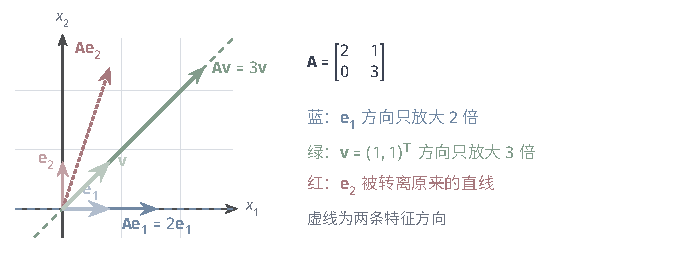
\includegraphics[width=112mm]{figures/00-shared/mathematical-preliminaries-upper/02-linear-spaces/tikz/comprehension-additions/operator-eigenvectors.pdf}
  \caption{特征向量只被伸缩、不被转向。算子$T(x_1,x_2)=(2x_1+x_2,3x_2)$在标准基下的矩阵为$\bm A=\left[\begin{smallmatrix}2&1\\0&3\end{smallmatrix}\right]$，它把$\bm e_1$送到$2\bm e_1$，把$\bm v=(1,1)^{\top}$送到$3\bm v$，二者都留在各自的虚线上；$\bm e_2$被送到$(1,3)^{\top}$，偏离了原来的直线，所以不是特征向量。}
  \label{fig:ls-operator-eigenvectors}
\end{figure}

并非每个算子都有实特征向量。下面的反例中，每个非零向量都被转离原来的直线。
\begin{example}[反例：平面旋转没有实特征向量]
\label{ex:ls-rotation-no-real-eigenvector}
给定平面上逆时针旋转$90^\circ$的算子$R(x_1,x_2)=(-x_2,x_1)$。检验它是否有实特征值。设实数$\lambda$与向量$(x_1,x_2)$满足$R(x_1,x_2)=\lambda(x_1,x_2)$，即
\[
 -x_2=\lambda x_1,\qquad x_1=\lambda x_2 .
\]
把第二式代入第一式得$-x_2=\lambda^2x_2$，即$(1+\lambda^2)x_2=0$。由于$1+\lambda^2>0$，只能$x_2=0$，进而$x_1=\lambda x_2=0$。结论：对任何实数$\lambda$，满足等式的只有零向量，所以$R$没有实特征值，也没有实特征向量。
\end{example}

\subsection{特征空间与不变子空间}

同一个特征值往往不止对应一条特征方向。固定特征值$\lambda$，满足$T\bm v=\lambda\bm v$的全部向量连同零向量组成集合$\ker(T-\lambda\,\operatorname{id}_V)$，称为$\lambda$的\term{特征空间}（eigenspace）。它是一个线性映射的核，因而是子空间。例如$\bm I_2$的每个非零向量都是属于$1$的特征向量，特征空间是整个平面；而示例~\ref{ex:ls-operator-eigenvector-check}中属于$2$的特征空间只是$\bm e_1$所在的直线，因为$\bm A-2\bm I=\left[\begin{smallmatrix}0&1\\0&1\end{smallmatrix}\right]$的核由第二坐标为零的向量组成。

特征空间是一类更一般的子空间的特例。若子空间$S$满足$T(S)\subseteq S$，就称$S$为$T$的\term{不变子空间}（invariant subspace）。这时作用不会把$S$中的向量带出$S$，于是可以把$T$限制在$S$上单独研究。特征空间是不变子空间，因为其中的向量只被乘以$\lambda$，仍留在其中。

一维不变子空间恰好就是特征方向。若$\bm v\neq\bm0$且$\operatorname{span}\{\bm v\}$不变，则$T\bm v$落在这条直线上，是$\bm v$的倍数；反之，若$T\bm v=\lambda\bm v$，则$T(c\bm v)=\lambda c\bm v$仍在这条直线上。高于一维的不变子空间却未必含有特征方向：整个平面对$90^\circ$旋转不变，而示例~\ref{ex:ls-rotation-no-real-eigenvector}说明其中没有一条特征方向。第~\ref{sec:ls-general-square-spectrum}节将看到，这样的二维不变子空间对应一对共轭的复特征值。

\subsection{特征多项式}
\label{sec:ls-characteristic-polynomial}

示例~\ref{ex:ls-operator-eigenvector-check}中的特征向量是先猜出、再验证的。能否系统地求出全部特征值？对$n$阶方阵$\bm A$，$\lambda$是特征值，当且仅当齐次方程$(\bm A-\lambda\bm I)\bm v=\bm0$有非零解，即$\ker(\bm A-\lambda\bm I)\neq\{\bm0\}$。由第~\ref{sec:ls-injective-surjective-invertible}节的等价条件，这又等价于$\operatorname{rank}(\bm A-\lambda\bm I)<n$，也等价于$\bm A-\lambda\bm I$不可逆。

不可逆又等价于行列式为零，这一步用到第~\ref{sec:ls-determinant-properties}节的两条性质。若方阵$\bm M$可逆，乘法性给出$\det\bm M\det(\bm M^{-1})=\det\bm I=1$，故$\det\bm M\neq0$；反之若$\det\bm M\neq0$，古典伴随恒等式说明$\operatorname{adj}(\bm M)/\det\bm M$就是$\bm M$的逆。所以$\lambda$是$\bm A$的特征值，当且仅当$\det(\bm A-\lambda\bm I)=0$。第~\ref{sec:ls-similarity-properties}节把每个$\operatorname{rank}(\bm A-c\bm I)$都列为相似不变量；现在可以看出，使这个秩小于$n$的数$c$恰好就是特征值。

为了把这个条件写成首项系数为正的多项式，注意$\det(\lambda\bm I-\bm A)=(-1)^n\det(\bm A-\lambda\bm I)$，二者同时为零。定义
\begin{equation}
 p_{\bm A}(z)=\det(z\bm I-\bm A),
 \label{eq:matrix-analysis-characteristic-polynomial}
\end{equation}
称为\term{特征多项式}（characteristic polynomial），就得到：$\bm A$的实特征值恰为$p_{\bm A}$的实根。在行列式的排列展开中，对角线一项是$\prod_i(z-a_{i,i})$；其余每一项至少有两个因子取自非对角位置，含$z$的因子至多$n-2$个。所以只有对角线一项含$z^n$，$p_{\bm A}$是首项系数为$1$的$n$次实多项式，至多有$n$个不同的根。求出一个特征值$\lambda$以后，再解齐次方程$(\bm A-\lambda\bm I)\bm v=\bm0$，就得到它的特征空间。

用特征多项式可以重新求出前面两个例子的特征值，而不必猜测特征向量。
\begin{example}[用特征多项式求特征值]
\label{ex:ls-characteristic-polynomial-two-by-two}
给定示例~\ref{ex:ls-operator-eigenvector-check}的$\bm A=\left[\begin{smallmatrix}2&1\\0&3\end{smallmatrix}\right]$，以及示例~\ref{ex:ls-rotation-no-real-eigenvector}的旋转在标准基下的矩阵$\bm R=\left[\begin{smallmatrix}0&-1\\1&0\end{smallmatrix}\right]$。二者的特征多项式为
\[
 \begin{aligned}
 p_{\bm A}(z)&=\det\begin{bmatrix}z-2&-1\\0&z-3\end{bmatrix}=(z-2)(z-3),\\
 p_{\bm R}(z)&=\det\begin{bmatrix}z&1\\-1&z\end{bmatrix}=z^2+1 .
 \end{aligned}
\]
结论：$\bm A$的特征值为$2$与$3$，与示例~\ref{ex:ls-operator-eigenvector-check}验证的两条特征方向相符；$z^2+1$对任何实数$z$都为正，没有实根，所以$\bm R$没有实特征值，与示例~\ref{ex:ls-rotation-no-real-eigenvector}的直接验证一致。
\end{example}
$\bm A$的情形可以推广到任意三角矩阵：三角矩阵$\bm A$的$z\bm I-\bm A$仍是三角矩阵，行列式是对角元之积$\prod_i(z-a_{i,i})$，所以三角矩阵的特征值就是它的对角元。

特征多项式在每个特征值处取零。若把矩阵本身代入特征多项式，又会得到什么？这里的代入是指把多项式中的$z^j$换成$\bm A^j$，常数项$c_0$换成$c_0\bm I$。先看一个例子。
\begin{example}[把矩阵代入它的特征多项式]
\label{ex:ls-cayley-hamilton-two-by-two}
给定$\bm A=\left[\begin{smallmatrix}2&1\\0&3\end{smallmatrix}\right]$。由示例~\ref{ex:ls-characteristic-polynomial-two-by-two}，$p_{\bm A}(z)=(z-2)(z-3)=z^2-5z+6$。计算$p_{\bm A}(\bm A)=\bm A^2-5\bm A+6\bm I$：
\[
 \bm A^2=\begin{bmatrix}4&5\\0&9\end{bmatrix},\qquad
 \bm A^2-5\bm A+6\bm I
 =\begin{bmatrix}4-10+6&5-5+0\\0&9-15+6\end{bmatrix}
 =\bm0 .
\]
结论：把$\bm A$代入自身的特征多项式，得到零矩阵。
\end{example}
这不是巧合。证明的工具是第~\ref{sec:ls-determinant-properties}节的古典伴随恒等式（定理~\ref{thm:ls-adjugate-identity}）$\bm M\operatorname{adj}(\bm M)=\det(\bm M)\bm I$。令$\bm M=z\bm I-\bm A$，得
\[
 (z\bm I-\bm A)\operatorname{adj}(z\bm I-\bm A)=p_{\bm A}(z)\bm I .
\]
$\operatorname{adj}(z\bm I-\bm A)$的每个元素都是$z\bm I-\bm A$的一个带符号的$n-1$阶余子式，它是$z$的多项式，次数不超过$n-1$。按$z$的幂次整理，可以写成$\operatorname{adj}(z\bm I-\bm A)=\sum_{j=0}^{n-1}z^j\bm B_j$，其中$\bm B_j$是不含$z$的常数矩阵。
\begin{theorem}[Cayley--Hamilton定理]
\label{thm:ls-cayley-hamilton}
设$n$阶方阵$\bm A$的特征多项式为$p_{\bm A}(z)=z^n+c_{n-1}z^{n-1}+\cdots+c_0$，则
\[
 p_{\bm A}(\bm A)
 =\bm A^n+c_{n-1}\bm A^{n-1}+\cdots+c_1\bm A+c_0\bm I=\bm0.
\]
\end{theorem}
\begin{proof}
把$\operatorname{adj}(z\bm I-\bm A)=\sum_{j=0}^{n-1}z^j\bm B_j$代入上式，左边为$\sum_jz^{j+1}\bm B_j-\sum_jz^j\bm A\bm B_j$。两边每个元素都是$z$的多项式，且对所有实数$z$相等，所以同次项的系数相等。记$c_n=1$，比较$z$的各次幂系数：
\[
 \begin{aligned}
 &z^n: &&\bm B_{n-1}=\bm I;\\
 &z^j\ (1\leq j\leq n-1): &&\bm B_{j-1}-\bm A\bm B_j=c_j\bm I;\\
 &z^0: &&-\bm A\bm B_0=c_0\bm I .
 \end{aligned}
\]
把$z^j$项的等式左乘$\bm A^j$（$j=0,\ldots,n$）后相加。右边恰为$\sum_jc_j\bm A^j=p_{\bm A}(\bm A)$；左边为
\[
 \bm A^n\bm B_{n-1}+\sum_{j=1}^{n-1}\bigl(\bm A^j\bm B_{j-1}-\bm A^{j+1}\bm B_j\bigr)-\bm A\bm B_0 ,
\]
其中相邻项逐对相消，总和为零。
\end{proof}
证明只用到行列式与古典伴随，既不需要先求出特征值，也不要求$p_{\bm A}$有实根。

定理的一个直接推论是，高次幂可以由低次幂表示。由$p_{\bm A}(\bm A)=\bm0$得$\bm A^n=-\sum_{j=0}^{n-1}c_j\bm A^j$，即$\bm A^n$是$\bm I,\bm A,\ldots,\bm A^{n-1}$的线性组合。两边再左乘$\bm A$，右端出现的$\bm A^n$同样用这个式子代换，可知$\bm A^{n+1}$也是这些矩阵的线性组合；归纳可得，所有$\bm A^k$（$k\geq n$）都是。因此，对任意向量$\bm g$，$\bm A^k\bm g$（$k\geq n$）都是$\bm g,\bm A\bm g,\ldots,\bm A^{n-1}\bm g$的线性组合，序列$\bm g,\bm A\bm g,\bm A^2\bm g,\ldots$张成的子空间在前$n$项之后不再增大。第~\ref{chap:linear-equations-and-optimization}章判断Sylvester方程何时有唯一解时，要用到这个定理。

同一个特征值可以是特征多项式的重根。这时，关于这个特征值有两种“个数”需要区分。根$\lambda$在$p_{\bm A}$中的重数称为\term{代数重数}（algebraic multiplicity），特征空间的维数$\dim\ker(\bm A-\lambda\bm I)$称为\term{几何重数}（geometric multiplicity）。下面的例子说明二者可以不同。
\begin{example}[代数重数大于几何重数]
\label{ex:ls-multiplicity-gap}
给定
\[
 \bm J=\begin{bmatrix}0.8&1\\0&0.8\end{bmatrix}.
\]
它是上三角矩阵，特征多项式为$p_{\bm J}(z)=(z-0.8)^2$，所以唯一的特征值$0.8$的代数重数为$2$。再求特征空间：
\[
 \bm J-0.8\bm I=\begin{bmatrix}0&1\\0&0\end{bmatrix},\qquad
 (\bm J-0.8\bm I)\begin{bmatrix}x_1\\x_2\end{bmatrix}=\begin{bmatrix}x_2\\0\end{bmatrix},
\]
它为零当且仅当$x_2=0$，所以特征空间是$(1,0)^{\top}$所在的直线。结论：特征值$0.8$的代数重数为$2$，几何重数只有$1$。
\end{example}
两种重数的一般关系，以及它们怎样决定能否找到由特征向量组成的基，在第~\ref{sec:ls-matrix-powers}节讨论。对一般的算子$T$，可以取任一组基把它写成矩阵，再求特征多项式与两种重数；下一小节说明，这样得到的结果不依赖基的选取。

\subsection{相似不变性}
\label{sec:ls-eigen-similarity-invariance}

第~\ref{sec:ls-similarity-properties}节列出了相似保持的量：秩、零空间的维数、每个$\operatorname{rank}(\bm A-c\bm I)$，以及行列式与迹。特征值、特征多项式与两种重数是否也在其中？若是，它们就属于算子本身，可以用任意一组基下的矩阵计算。下面设$\bm B=\bm P^{-1}\bm A\bm P$，其中$\bm P$可逆。

先看特征值与几何重数。若$\bm A\bm v=\lambda\bm v$且$\bm v\neq\bm0$，则
\[
 \bm B(\bm P^{-1}\bm v)=\bm P^{-1}\bm A\bm P\bm P^{-1}\bm v=\bm P^{-1}\bm A\bm v=\lambda\bm P^{-1}\bm v .
\]
$\bm P$可逆保证$\bm P^{-1}\bm v\neq\bm0$，所以$\lambda$也是$\bm B$的特征值，相应的特征向量是$\bm P^{-1}\bm v$；交换$\bm A,\bm B$的角色即得反向结论。同样的计算说明$\ker(\bm B-\lambda\bm I)=\bm P^{-1}\ker(\bm A-\lambda\bm I)$，而可逆矩阵把子空间映成同维数的子空间，所以每个特征值的几何重数不变。这一结论也可以由式~\eqref{eq:ls-similarity-shifted-rank}取$c=\lambda$、再用秩零度定理换成核的维数得到。

更进一步，整个特征多项式不变：
\[
 p_{\bm B}(z)=\det(z\bm I-\bm P^{-1}\bm A\bm P)=\det\bigl(\bm P^{-1}(z\bm I-\bm A)\bm P\bigr)=p_{\bm A}(z),
\]
中间一步用了$z\bm I=\bm P^{-1}(z\bm I)\bm P$，最后一步用了第~\ref{sec:ls-similarity-properties}节的恒等式$\det(\bm P^{-1}\bm M\bm P)=\det\bm M$。所以算子的特征多项式可以用任意一组基下的矩阵计算，代数重数也是相似不变量。

特征多项式的系数还说明了行列式与迹为什么是相似不变量：它们就是$p_{\bm A}$的两个系数，至多差一个符号。令$z=0$，得常数项$p_{\bm A}(0)=\det(-\bm A)=(-1)^n\det\bm A$。再看$z^{n-1}$的系数。上一小节已经指出，排列展开中除对角线一项外，每一项含$z$的因子至多$n-2$个；所以$z^{n-1}$只来自$\prod_i(z-a_{i,i})$，系数为$-\sum_ia_{i,i}=-\operatorname{tr}\bm A$。于是
\[
 p_{\bm A}(z)=z^n-(\operatorname{tr}\bm A)\,z^{n-1}+\cdots+(-1)^n\det\bm A .
\]

若$p_{\bm A}$能分解为实一次因子之积$\prod_{i=1}^n(z-\lambda_i)$，其中每个特征值按代数重数重复列出，把右端展开后比较$z^{n-1}$的系数与常数项，得
\[
 \operatorname{tr}\bm A=\sum_{i=1}^n\lambda_i,\qquad \det\bm A=\prod_{i=1}^n\lambda_i .
\]
例如示例~\ref{ex:ls-operator-eigenvector-check}的$\bm A$有$\operatorname{tr}\bm A=5=2+3$，$\det\bm A=6=2\cdot3$。第~\ref{sec:ls-general-square-spectrum}节把特征多项式的复根也算作特征值以后，这两个等式对每个方阵都成立。

相似不变量只能用来否定相似：某个相似不变量不同，两个矩阵就不相似；不变量全部相同，两个矩阵却未必相似。第~\ref{sec:ls-similarity-conditions}节比较过$\bm I_2$与$\left[\begin{smallmatrix}1&1\\0&1\end{smallmatrix}\right]$，现在可以用特征值的语言重新说明二者为什么不相似。
\begin{example}[反例：特征多项式相同而不相似]
\label{ex:ls-same-charpoly-not-similar}
给定$\bm I_2$与
\[
 \bm J_1=\begin{bmatrix}1&1\\0&1\end{bmatrix}.
\]
二者都是上三角矩阵，对角元都是$1$，所以$p_{\bm I_2}(z)=p_{\bm J_1}(z)=(z-1)^2$，特征值$1$的代数重数都是$2$。另一方面，
\[
 \bm I_2-\bm I_2=\bm0,\qquad
 \bm J_1-\bm I_2=\begin{bmatrix}0&1\\0&0\end{bmatrix},
\]
前者的核是整个平面，后者的核只是$(1,0)^{\top}$所在的直线，几何重数分别为$2$与$1$。结论：二者的特征多项式相同，但几何重数不同；由于几何重数是相似不变量，它们不相似。
\end{example}
所以特征多项式相同只是相似的必要条件。比较各特征值的几何重数是更细的必要条件，但一般仍不足以判定相似；完整的相似分类需要Jordan标准形，本书不展开。下一节只处理最重要、也最常用的一类矩阵：与对角矩阵相似的矩阵。

\subsection{不同特征值的特征向量}
\label{sec:ls-eigenvector-independence}

特征方向能否多到组成一组基？先要说明，属于不同特征值的特征向量不会彼此重复，即它们线性无关。设$\bm v_1,\ldots,\bm v_r$分别属于互不相同的特征值$\lambda_1,\ldots,\lambda_r$，假设它们线性相关。在所有非平凡的线性依赖中取项数最少的一个，重新编号后记为$\sum_{j=1}^s c_j\bm v_j=\bm0$，其中各$c_j\neq0$；单个特征向量非零，不能单独构成依赖，所以$s\geq2$。两边作用$T-\lambda_1\operatorname{id}_V$：第一项变为零，其余各项变为$c_j(\lambda_j-\lambda_1)\bm v_j$。特征值互不相同，这些系数仍非零，于是得到一个只有$s-1$项的非平凡依赖，与$s$最少矛盾。所以$\bm v_1,\ldots,\bm v_r$线性无关。由于$n$维空间中线性无关的向量至多$n$个，$n$维空间上的算子至多有$n$个不同特征值，这与特征多项式的次数给出的上界一致。

由此，不同特征值的特征空间之和是直和。设$\sum_\lambda\bm w_\lambda=\bm0$，每个$\bm w_\lambda$属于相应的特征空间；其中非零的$\bm w_\lambda$是属于不同特征值的特征向量，它们线性无关，所以只能每个$\bm w_\lambda=\bm0$。把各特征空间的基合在一起，它们的任一线性组合都可以按特征值分组写成$\sum_\lambda\bm w_\lambda$；若组合为零，则每个$\bm w_\lambda=\bm0$，而每组基本身线性无关，所以全部系数为零。因此各特征空间的基合在一起仍线性无关。例如示例~\ref{ex:ls-operator-eigenvector-check}中的$\bm e_1$与$(1,1)^{\top}$属于不同的特征值$2$与$3$，不必另行验证，它们自动线性无关，在平面上组成一组基。

至此，本节开头的四个问题都有了回答。被算子只伸缩的方向是特征方向，伸缩倍数是特征值；特征值是特征多项式的实根，求出特征值后解齐次方程即得特征空间。特征值、特征多项式和两种重数都不随基改变，属于算子本身。属于不同特征值的特征向量线性无关，所以$n$维空间上的算子至多有$n$个不同特征值。途中还得到了Cayley--Hamilton定理：$\bm A$的高次幂都能用$\bm I,\bm A,\ldots,\bm A^{n-1}$表示。剩下的问题是特征向量什么时候多到足以组成一组基，这是下一节的对角化问题。

% 第6章第2节：基于可逆矩阵的对角化（特征基下的矩阵与幂、可对角化的定义与判据及不能对角化的情形、步骤与算例）。

\section{基于可逆矩阵的对角化}
\label{sec:ls-matrix-powers}
\label{sec:ch06-powers-spectrum}

上一节找到了被算子只伸缩的方向，并证明属于不同特征值的特征向量线性无关。本节回答由此引出的问题：有了由特征向量组成的基，算子的矩阵变成什么样，又能怎样利用？这样的基什么时候存在？换到这组基所用的换基矩阵只要求可逆，不要求各列互相垂直，所以本节的对角化是用一般的可逆矩阵作相似变换。

\subsection{特征基下的矩阵}
\label{sec:matrix-analysis-spectrum}

设$\bm v_1,\ldots,\bm v_n$是由算子$T$的特征向量组成的基，$T\bm v_j=\lambda_j\bm v_j$。按第~\ref{sec:ls-map-representation}节的约定，$T$在这组基下的矩阵的第$j$列是$T\bm v_j=\lambda_j\bm v_j$的坐标，即第$j$个位置为$\lambda_j$、其余位置为零。所以这个矩阵在主对角线以外全为零，每个基方向被独立地伸缩。示例~\ref{ex:ls-operator-eigenvector-check}中的$(\bm e_1,(1,1)^{\top})$就是这样一组基。换到这组基，正是第~\ref{sec:ls-similarity}节的相似变换$\bm P^{-1}\bm A\bm P=\operatorname{diag}(2,3)$；在图~\ref{fig:ls-similarity-change-of-basis-flow}中，基向量围成的平行四边形只沿两条特征方向分别伸长$2$倍和$3$倍。

这一观察也可以写成矩阵等式。设$\bm A$是$T$在标准基下的矩阵，把特征向量的标准坐标排成$\bm V=[\bm v_1,\ldots,\bm v_n]$。$\bm V$的各列是新基向量的旧坐标，所以它正是第~\ref{sec:ls-similarity}节的换基矩阵；各列线性无关，所以$\bm V$可逆（第~\ref{sec:ls-injective-surjective-invertible}节）。按乘积的列读法，$\bm A\bm V$的第$j$列是$\bm A\bm v_j=\lambda_j\bm v_j$；右乘对角矩阵$\bm\Lambda=\operatorname{diag}(\lambda_1,\ldots,\lambda_n)$把第$j$列乘以$\lambda_j$，所以$\bm V\bm\Lambda$的第$j$列也是$\lambda_j\bm v_j$。于是$\bm A\bm V=\bm V\bm\Lambda$，两边左乘或右乘$\bm V^{-1}$，即得
\[
 \bm V^{-1}\bm A\bm V=\bm\Lambda,\qquad \bm A=\bm V\bm\Lambda\bm V^{-1}.
\]

对角形式的好处在反复作用时最明显。同一个方阵反复作用，是矩阵乘法最常见的用法之一：定常迭代$\bm x^{(k+1)}=\bm A\bm x^{(k)}$走$k$步后得到$\bm x^{(k)}=\bm A^k\bm x^{(0)}$。第~\ref{sec:ls-matrix-power-rules}节规定了矩阵幂的写法，但直接连乘会不断混合各个坐标，看不出$\bm A^k$在$k$很大时是什么样子。把$\bm A=\bm V\bm\Lambda\bm V^{-1}$连乘$k$次，相邻的$\bm V^{-1}\bm V$相消（这就是式~\eqref{eq:ls-similarity-product}后面的$\bm B^k=\bm P^{-1}\bm A^k\bm P$），得到
\begin{equation}
 \bm A^k=\bm V\bm\Lambda^k\bm V^{-1},\qquad
 \bm\Lambda^k=\operatorname{diag}(\lambda_1^k,\ldots,\lambda_n^k).
 \label{eq:ls-diagonalization-power}
\end{equation}
于是求幂只需对对角元逐个乘方。三个因子可以从右向左读：$\bm V^{-1}\bm x^{(0)}$给出初值在各特征方向上的坐标，$\bm\Lambda^k$把第$j$个坐标乘以$\lambda_j^k$，$\bm V$再把结果合回标准坐标。上一节已经看到，沿特征方向有$\bm A^k\bm v=\lambda^k\bm v$；式~\eqref{eq:ls-diagonalization-power}把这一点推广到任意初值。

下面用一个上三角矩阵演示这种计算：先把一个初值拆成特征方向上的分量，再对所有初值一并写出矩阵幂。
\begin{example}[用特征向量计算矩阵幂]
\label{ex:ls-triangular-power}
给定
\[
 \bm A=\begin{bmatrix}0.8&4\\0&0.5\end{bmatrix},
\]
计算$\bm A^k$。

第一步，求特征值与特征向量。$\bm A$是上三角矩阵，特征值为对角元$0.8$与$0.5$。直接验证
\[
 \bm A\begin{bmatrix}1\\0\end{bmatrix}=0.8\begin{bmatrix}1\\0\end{bmatrix},\qquad
 \bm A\begin{bmatrix}-40/3\\1\end{bmatrix}
 =\begin{bmatrix}-32/3+4\\0.5\end{bmatrix}
 =0.5\begin{bmatrix}-40/3\\1\end{bmatrix},
\]
所以$\bm v_1=(1,0)^{\top}$与$\bm v_2=(-40/3,1)^{\top}$是特征向量。

第二步，计算一条轨迹。初值$(0,1)^{\top}$不在特征方向上，先把它拆成$(0,1)^{\top}=\tfrac{40}{3}\bm v_1+\bm v_2$。两个分量每作用一次分别乘以$0.8$与$0.5$，由线性性，
\[
 \bm A^k\begin{bmatrix}0\\1\end{bmatrix}
 =\frac{40}{3}\,0.8^k\bm v_1+0.5^k\bm v_2
 =\begin{bmatrix}\tfrac{40}{3}(0.8^k-0.5^k)\\0.5^k\end{bmatrix}.
\]
$k=1$时得$(4,0.5)^{\top}$，与直接计算$\bm A(0,1)^{\top}$一致。

第三步，对所有初值一并计算，即应用式~\eqref{eq:ls-diagonalization-power}。取$\bm V=\left[\begin{smallmatrix}1&-40/3\\0&1\end{smallmatrix}\right]$，则$\bm V^{-1}=\left[\begin{smallmatrix}1&40/3\\0&1\end{smallmatrix}\right]$，
\[
 \bm A^k=\bm V\begin{bmatrix}0.8^k&0\\0&0.5^k\end{bmatrix}\bm V^{-1}
 =\begin{bmatrix}0.8^k&\tfrac{40}{3}(0.8^k-0.5^k)\\0&0.5^k\end{bmatrix}.
\]
结论：$\bm A^k$的第二列正是第二步的轨迹；整个迭代拆成两个独立的数列，分别按$0.8^k$与$0.5^k$衰减。
\end{example}
这种计算依赖一个前提：特征向量足以组成整个空间的一组基。下一小节讨论这个前提何时成立。

\subsection{可对角化的定义与判据}

\paragraph{定义与特征向量判据}
上一小节说明，有了由特征向量组成的基，$\bm A$就相似于一个对角矩阵。把相似于对角矩阵这一性质取作定义。
\begin{definition}[实可对角化]
\label{def:ls-real-diagonalizable}
设$\bm A$是$n$阶实方阵。若存在$n$阶实可逆矩阵$\bm V$与实对角矩阵$\bm\Lambda$使$\bm V^{-1}\bm A\bm V=\bm\Lambda$，即$\bm A$相似于实对角矩阵，就称$\bm A$\term{实可对角化}（diagonalizable over the reals）；求出这样的$\bm V$与$\bm\Lambda$，称为把$\bm A$对角化。
\end{definition}
“实”表示$\bm V$与$\bm\Lambda$的元素都是实数。本书在实数范围内讨论，下文所说的可对角化都指实可对角化。

哪些矩阵可以对角化？下面的判据把问题化为特征向量够不够多。
\begin{theorem}[对角化判据]
\label{thm:ls-diagonalization-criterion}
$n$阶实方阵$\bm A$实可对角化，当且仅当$\bm A$有$n$个线性无关的实特征向量。这时以这些特征向量为列组成$\bm V$，以相应特征值按同一顺序组成$\bm\Lambda=\operatorname{diag}(\lambda_1,\ldots,\lambda_n)$，就有$\bm V^{-1}\bm A\bm V=\bm\Lambda$。
\end{theorem}
\begin{proof}
设$\bm V$的各列为$\bm v_1,\ldots,\bm v_n$，$\bm\Lambda=\operatorname{diag}(\lambda_1,\ldots,\lambda_n)$。上一小节的列读法对任意这样的$\bm V$与$\bm\Lambda$都成立，它给出
\[
 \bm A\bm V=\bm V\bm\Lambda
 \quad\Longleftrightarrow\quad
 \bm A\bm v_j=\lambda_j\bm v_j,\qquad j=1,\ldots,n.
\]
若$\bm A$有$n$个线性无关的特征向量，以它们为列的$\bm V$可逆，左乘$\bm V^{-1}$即得$\bm V^{-1}\bm A\bm V=\bm\Lambda$。反过来，若$\bm V^{-1}\bm A\bm V=\bm\Lambda$，左乘$\bm V$得$\bm A\bm V=\bm V\bm\Lambda$，于是每列都满足$\bm A\bm v_j=\lambda_j\bm v_j$；$\bm V$可逆，所以各列线性无关，从而都非零，它们是$n$个线性无关的特征向量。
\end{proof}
由第~\ref{sec:ls-eigenvector-independence}节，属于不同特征值的特征向量线性无关，由此得到一个常用的充分条件：$n$阶实方阵若有$n$个互不相同的实特征值，就实可对角化。示例~\ref{ex:ls-triangular-power}的矩阵即属此类。这个条件不是必要的：单位矩阵$\bm I_n$只有一个特征值$1$，本身却已经是对角矩阵。

\paragraph{不能对角化的矩阵}
判据要求$n$个线性无关的实特征向量，这一要求可能在两处得不到满足。其一，实特征值不够。示例~\ref{ex:ls-rotation-no-real-eigenvector}与示例~\ref{ex:ls-characteristic-polynomial-two-by-two}已经说明，平面上的$90^\circ$旋转$\bm R=\left[\begin{smallmatrix}0&-1\\1&0\end{smallmatrix}\right]$没有实特征值，也就没有实特征向量，所以不能实对角化。其二，实特征值有了，特征向量却不够。示例~\ref{ex:ls-multiplicity-gap}中的$\bm J=\left[\begin{smallmatrix}0.8&1\\0&0.8\end{smallmatrix}\right]$只有特征值$0.8$，而特征向量只有$(1,0)^{\top}$的倍数，凑不出两个线性无关的特征向量，所以$\bm J$也不能对角化。

对这样的矩阵，式~\eqref{eq:ls-diagonalization-power}不再可用，幂也不再是纯粹的乘方。下面直接计算$\bm J^k$。
\begin{example}[不能对角化矩阵的幂]
\label{ex:ls-jordan-block-power}
给定$\bm J=\left[\begin{smallmatrix}0.8&1\\0&0.8\end{smallmatrix}\right]$，计算$\bm J^k$。把$\bm J$写成$0.8\bm I+\bm N$，其中
\[
 \bm N=\begin{bmatrix}0&1\\0&0\end{bmatrix},\qquad \bm N^2=\bm0 .
\]
$0.8\bm I$与$\bm N$可交换，所以二项式展开成立；又因为$j\geq2$时$\bm N^j=\bm0$，展开后只剩前两项：
\[
 \bm J^k=(0.8\bm I+\bm N)^k=0.8^k\bm I+k\,0.8^{k-1}\bm N=\begin{bmatrix}0.8^k&k\,0.8^{k-1}\\0&0.8^k\end{bmatrix}.
\]
右上角相邻两项之比为$\dfrac{(k+1)\,0.8^{k}}{k\,0.8^{k-1}}=0.8\cdot\dfrac{k+1}{k}$，它在$k<4$时大于$1$，在$k>4$时小于$1$。结论：右上角的$k\,0.8^{k-1}$随$k$先增大、后衰减，不能由单个特征值的乘方描述。
\end{example}

\paragraph{重数判据}
两个反例分别缺了什么？$\bm R$的特征多项式$z^2+1$不能分解为实一次因子；$\bm J$的特征多项式$(z-0.8)^2$分解了，但特征值$0.8$的几何重数$1$小于代数重数$2$。下面说明，这两种缺陷恰好是全部障碍。于是能否对角化可以直接由特征多项式和特征空间的维数判断，而不必逐个尝试特征向量。

先证明几何重数不超过代数重数。设特征值$\lambda$的特征空间维数为$g$，取它的一组基，并扩充成全空间的一组基。在新基下，前$g$个基向量都被送到自身的$\lambda$倍，所以$\bm A$相似于分块上三角矩阵$\left[\begin{smallmatrix}\lambda\bm I_g&*\\\bm0&\bm C\end{smallmatrix}\right]$。相似不改变特征多项式（第~\ref{sec:ls-eigen-similarity-invariance}节），所以可以用这个分块矩阵计算$p_{\bm A}$。用$z\bm I$减去它以后，前$g$列都只在对角位置上有非零元素$z-\lambda$。沿第一列按余子式展开（第~\ref{sec:ls-determinant-properties}节），得到$z-\lambda$乘以一个形状相同、但只剩$g-1$个这种列的行列式；重复$g$次，即得$p_{\bm A}(z)=(z-\lambda)^g\,p_{\bm C}(z)$。所以代数重数至少为$g$。示例~\ref{ex:ls-multiplicity-gap}说明不等号可以严格成立。

由此得到可以计算的判据：$\bm A$实可对角化，当且仅当$p_{\bm A}$能分解为实一次因子之积，且每个特征值的几何重数等于代数重数。

先证充分性。$p_{\bm A}$分解为$n$个实一次因子时，各特征值的代数重数之和为$n$；几何重数与代数重数逐个相等，所以几何重数之和也是$n$。由第~\ref{sec:ls-eigenvector-independence}节，不同特征值的特征空间之和是直和，各特征空间的基合在一起仍线性无关，于是恰好得到$n$个线性无关的特征向量；由对角化判据，$\bm A$可对角化。

再证必要性。若$\bm A=\bm V\bm\Lambda\bm V^{-1}$，则由相似不变性，$p_{\bm A}=p_{\bm\Lambda}=\prod_i(z-\lambda_i)$已分解为实一次因子。对每个特征值$\lambda$，它在$\bm\Lambda$对角线上出现的次数既是代数重数，也是$\bm\Lambda-\lambda\bm I$的零空间维数，即$\bm\Lambda$的几何重数。由第~\ref{sec:ls-eigen-similarity-invariance}节，相似不改变几何重数，所以$\bm A$的两种重数也相等。

有$n$个互不相同的实特征值时，每个代数重数都是$1$，几何重数至少为$1$又不超过$1$，判据的条件自动满足，这就回到了前面的充分条件。

\subsection{对角化的步骤与算例}

按判据，对角化分四步。第一步，求出特征多项式$p_{\bm A}$的全部实根，即全部实特征值。第二步，对每个特征值$\lambda$解齐次方程$(\bm A-\lambda\bm I)\bm v=\bm0$，得到特征空间的一组基。第三步，若这些向量合起来共有$n$个，就以它们为列组成$\bm V$，以对应的特征值按同一顺序组成$\bm\Lambda$。第四步，核对$\bm A\bm V=\bm V\bm\Lambda$。若特征多项式不能分解为实一次因子，或某个特征空间的维数小于相应的代数重数，过程就在第一步或第三步停止，矩阵不能实对角化，这正是上一小节的两种情形。

下面用一个两状态转移的例子走一遍这四步。设一个群体在两个状态之间转移：每期处于状态一的个体有$10\%$转入状态二，处于状态二的个体有$20\%$转入状态一。记第$k$期两个状态所占的比例为$\bm x^{(k)}=(x_1^{(k)},x_2^{(k)})^{\top}$，则下一期状态一的比例为$0.9x_1^{(k)}+0.2x_2^{(k)}$，状态二的比例为$0.1x_1^{(k)}+0.8x_2^{(k)}$，即
\[
 \bm x^{(k+1)}=\bm A\bm x^{(k)},\qquad
 \bm A=\begin{bmatrix}0.9&0.2\\0.1&0.8\end{bmatrix}.
\]
\begin{example}[两状态转移矩阵的对角化]
\label{ex:ls-transition-matrix-diagonalization}
给定转移矩阵$\bm A=\left[\begin{smallmatrix}0.9&0.2\\0.1&0.8\end{smallmatrix}\right]$，按四步把它对角化。

第一步，求特征值：
\[
 p_{\bm A}(z)=(z-0.9)(z-0.8)-0.2\cdot0.1=z^2-1.7z+0.7=(z-1)(z-0.7),
\]
得$\lambda_1=1$、$\lambda_2=0.7$。两个特征值不同，所以$\bm A$可对角化。

第二步，求特征空间。$\lambda_1=1$时$\bm A-\bm I=\left[\begin{smallmatrix}-0.1&0.2\\0.1&-0.2\end{smallmatrix}\right]$，两行成比例，方程化为$-0.1x_1+0.2x_2=0$，取$\bm v_1=(2,1)^{\top}$。$\lambda_2=0.7$时$\bm A-0.7\bm I=\left[\begin{smallmatrix}0.2&0.2\\0.1&0.1\end{smallmatrix}\right]$，方程化为$x_1+x_2=0$，取$\bm v_2=(1,-1)^{\top}$。

第三步，组成
\[
 \bm V=\begin{bmatrix}2&1\\1&-1\end{bmatrix},\qquad
 \bm\Lambda=\begin{bmatrix}1&0\\0&0.7\end{bmatrix},\qquad
 \bm V^{-1}=\frac13\begin{bmatrix}1&1\\1&-2\end{bmatrix},
\]
其中$\bm V^{-1}$由二阶逆矩阵公式得到，$\det\bm V=-3$。

第四步，核对：
\[
 \bm A\bm v_1=\begin{bmatrix}1.8+0.2\\0.2+0.8\end{bmatrix}=\bm v_1,\qquad
 \bm A\bm v_2=\begin{bmatrix}0.9-0.2\\0.1-0.8\end{bmatrix}=0.7\bm v_2,
\]
所以$\bm A\bm V=\bm V\bm\Lambda$。也可以用上一节的系数关系作快速检查：$\operatorname{tr}\bm A=1.7=1+0.7$，$\det\bm A=0.7=1\cdot0.7$。

结论：$\bm A=\bm V\bm\Lambda\bm V^{-1}$，$\bm V$的两列分别是属于特征值$1$与$0.7$的特征向量。
\end{example}

有了这个分解，就可以按式~\eqref{eq:ls-diagonalization-power}回答这个群体的长期去向。
\begin{example}[转移矩阵的长期比例]
\label{ex:ls-transition-matrix-long-run}
沿用示例~\ref{ex:ls-transition-matrix-diagonalization}的分解，计算$\bm A^k$以及$k\to\infty$时两个状态的比例。由式~\eqref{eq:ls-diagonalization-power}，
\[
 \bm A^k=\bm V\begin{bmatrix}1&0\\0&0.7^k\end{bmatrix}\bm V^{-1}
 =\frac13\begin{bmatrix}2+0.7^k&2-2\cdot0.7^k\\1-0.7^k&1+2\cdot0.7^k\end{bmatrix};
\]
$k=1$时右端正是$\bm A$。若开始时全部个体处于状态一，即$\bm x^{(0)}=(1,0)^{\top}$，则$\bm x^{(k)}$是$\bm A^k$的第一列：
\[
 \bm x^{(k)}=\frac13\begin{bmatrix}2+0.7^k\\1-0.7^k\end{bmatrix}
 \to\begin{bmatrix}2/3\\1/3\end{bmatrix}\qquad(k\to\infty).
\]
对一般的初始比例$\bm x^{(0)}=(a,1-a)^{\top}$，$\bm V^{-1}\bm x^{(0)}$给出它在两条特征方向上的分量：
\[
 \bm V^{-1}\bm x^{(0)}=\frac13\begin{bmatrix}a+(1-a)\\a-2(1-a)\end{bmatrix}=\begin{bmatrix}1/3\\(3a-2)/3\end{bmatrix}.
\]
沿$\bm v_1$的分量总是$1/3$，沿$\bm v_2$的分量每期乘以$0.7$而趋于零。结论：无论从什么比例出发，长期比例都是$\tfrac13\bm v_1=(2/3,1/3)^{\top}$。
\end{example}

至此，本节开头的问题有了回答。在由特征向量组成的基下，算子的矩阵是对角的；以特征向量为列的$\bm V$把$\bm A$化为$\bm\Lambda$，反复作用化为特征值的乘方，$\bm A^k=\bm V\bm\Lambda^k\bm V^{-1}$。$n$阶矩阵可对角化，当且仅当它有$n$个线性无关的实特征向量；等价地，特征多项式分解为实一次因子，且每个特征值的几何重数等于代数重数。实特征值不足或特征向量不足时，矩阵不能对角化；后一种情形的幂含有随$k$增长的多项式因子。

对角化回答了“能否找到只被伸缩的基方向”，却没有要求这些方向互相垂直。示例~\ref{ex:ls-transition-matrix-diagonalization}中的两条特征方向$(2,1)^{\top}$与$(1,-1)^{\top}$内积为$1$，并不垂直。换到这样的基，求新坐标要解方程，新坐标的平方和也不等于原向量长度的平方。下一节追问，哪些矩阵能用正交矩阵对角化，即具有一组标准正交的特征向量。至于不能对角化的矩阵在标准正交基下能化到多简单，以及特征向量接近线性相关时矩阵幂有多大，分别留给第~\ref{sec:ls-general-square-spectrum}节与第~\ref{sec:ls-matrix-power-behavior}节。

% 第6章第3节：基于正交矩阵的对角化（谱定理、Rayleigh商与谱的极值性质、对称矩阵的函数）。

\section{基于正交矩阵的对角化}
\label{sec:ls-spectral-theory}

上一节用可逆矩阵$\bm V$对角化，只要求基由特征向量组成，没有要求这些方向互相垂直。本节追问：哪些矩阵能用正交矩阵对角化，即找到一组标准正交的特征向量？答案是实对称矩阵，这一结论称为谱定理。有了这种分解，特征值还获得第二种含义：它们是二次型在单位球面上的极值，因此可以不求特征向量而比较、估计特征值。沿互相垂直的特征方向，还可以定义矩阵的平方根、对数等函数。

\subsection{谱定理}
\label{sec:ls-symmetric-spectral-decomposition}

先说明为什么希望特征方向互相垂直。若$\bm q_1,\ldots,\bm q_d$是$\mathbb R^d$的标准正交基，把它们排成正交矩阵$\bm Q$，则$\bm Q^{-1}=\bm Q^\top$。于是换基不必解方程：向量$\bm x$的新坐标就是内积$c_i=\bm q_i^\top\bm x$，长度也保持不变，$\lVert\bm x\rVert_2^2=\sum_ic_i^2$（第~\ref{sec:ls-orthonormal-bases}节）。所以，若方阵$\bm A$能写成$\bm A=\bm Q\bm\Lambda\bm Q^\top$，其中$\bm\Lambda$为实对角矩阵，它的作用就最容易看清：先用内积读出各方向的坐标，再把第$i$个坐标乘以$\lambda_i$，最后合回去。

哪些矩阵能这样写？必要条件很容易看出：若$\bm A=\bm Q\bm\Lambda\bm Q^\top$，则$\bm A^\top=\bm Q\bm\Lambda^\top\bm Q^\top=\bm A$，所以$\bm A$必须对称。对称矩阵也就是第~\ref{sec:ls-adjoints}节的自伴算子在标准坐标下的矩阵。本小节证明这一条件也是充分的。

下面把对称矩阵记为$\bm S$。证明的思路是：在单位球面上最大化二次型$\bm x^\top\bm S\bm x$，说明取到最大值的方向是一个特征方向，再在与它垂直的子空间中重复这一步。为此先要确认最大值确实能取到。

二次型在单位球面上有界：单位向量的每个坐标满足$|x_i|\leq1$，所以$|\bm x^\top\bm S\bm x|\leq\sum_{i,j}|s_{i,j}||x_i||x_j|\leq\sum_{i,j}|s_{i,j}|$。由确界原理，它有上确界$M$。取单位向量序列$\bm x_k$使$\bm x_k^\top\bm S\bm x_k\to M$，记$\bm x_k$的第$i$个坐标为$x_{k,i}$，各坐标数列都在$[-1,1]$中。由有界数列必有收敛子列（定理~\ref{thm:analysis-bounded-subsequence}），先取子列使第一个坐标收敛，再在这个子列中取子列使第二个坐标收敛，如此进行$d$次，得到一个每个坐标都收敛的子列，记其极限为$\bm x_*$。沿这个子列取极限，由极限的四则运算得$\lVert\bm x_*\rVert_2^2=\lim\sum_ix_{k,i}^2=1$与$\bm x_*^\top\bm S\bm x_*=\lim\bm x_k^\top\bm S\bm x_k=M$。所以$M$在单位球面上的点$\bm x_*$处取到，是最大值。

从这个最大点出发，逐个找出互相正交的特征方向，就得到下面的结论，称为\term{谱定理}（spectral theorem）。

\begin{theorem}[谱定理]
\label{thm:ls-real-symmetric-spectral}
\label{thm:matrix-analysis-symmetric-spectral-theorem}
\label{sec:ch06-triangular-spectrum}
设$\bm S\in\mathbb R^{d\times d}$满足$\bm S=\bm S^\top$，则存在正交矩阵$\bm Q=[\bm q_1,\ldots,\bm q_d]$与实对角矩阵$\bm\Lambda=\operatorname{diag}(\lambda_1,\dots,\lambda_d)$，使
\begin{equation}
 \bm S=\bm Q\bm\Lambda\bm Q^\top,
 \qquad \bm S\bm q_i=\lambda_i\bm q_i.
 \label{eq:matrix-analysis-symmetric-eigendecomposition}
\end{equation}
对任意$\bm x=\sum_i c_i\bm q_i$，二次型展开为
\begin{equation}
 \bm x^\top\bm S\bm x=\sum_{i=1}^d\lambda_i c_i^2.
 \label{eq:matrix-analysis-quadratic-spectral-form}
\end{equation}
\end{theorem}

\begin{proof}
分三步。

第一步，找出最大方向。由定理前的论证，二次型$q(\bm x)=\bm x^\top\bm S\bm x$在单位球面上取到最大值，记最大值为$\lambda_1$、最大点为$\bm q_1$。对任意$\bm x\neq\bm0$，$\bm x/\lVert\bm x\rVert_2$在单位球面上，而$q$是二次齐次的，所以
\[
 q(\bm x)=\lVert\bm x\rVert_2^2\,q\bigl(\bm x/\lVert\bm x\rVert_2\bigr)\leq\lambda_1\lVert\bm x\rVert_2^2 .
\]

第二步，说明$\bm q_1$是特征向量。任取与$\bm q_1$正交的$\bm h$和实数$t$，把$\bm x=\bm q_1+t\bm h$代入上面的不等式。由勾股定理$\lVert\bm q_1+t\bm h\rVert_2^2=1+t^2\lVert\bm h\rVert_2^2$；又由$\bm S$对称，$\bm q_1^\top\bm S\bm h=\bm h^\top\bm S\bm q_1$，于是
\[
 \lambda_1+2t\,\bm h^\top\bm S\bm q_1+t^2\bm h^\top\bm S\bm h
 \leq\lambda_1+t^2\lambda_1\lVert\bm h\rVert_2^2 ,
\]
即$2t\,\bm h^\top\bm S\bm q_1\leq t^2c$，其中$c=\lambda_1\lVert\bm h\rVert_2^2-\bm h^\top\bm S\bm h$。取$t>0$，两边除以$t$得$2\bm h^\top\bm S\bm q_1\leq tc$，令$t\to0^+$得$\bm h^\top\bm S\bm q_1\leq0$；取$t<0$，除以$t$时不等号反向，令$t\to0^-$得$\bm h^\top\bm S\bm q_1\geq0$。所以$\bm h^\top\bm S\bm q_1=0$。这对所有$\bm h\perp\bm q_1$成立，说明$\bm S\bm q_1$在$\bm q_1$的正交补中没有分量，只能是$\bm q_1$的倍数：$\bm S\bm q_1=(\bm q_1^\top\bm S\bm q_1)\bm q_1=\lambda_1\bm q_1$。

第三步，对正交补归纳。对$\bm h\perp\bm q_1$，$\bm q_1^\top(\bm S\bm h)=(\bm S\bm q_1)^\top\bm h=\lambda_1\bm q_1^\top\bm h=0$，所以$\bm S$把$d-1$维子空间$\bm q_1^\perp$映到自身；对其中任意$\bm u,\bm v$仍有$\bm u^\top\bm S\bm v=\bm v^\top\bm S\bm u$，在$\bm q_1^\perp$的标准正交基下，$\bm S$的作用由一个$d-1$阶对称矩阵表示。对它重复前两步，得到$\bm q_2\perp\bm q_1$与$\lambda_2$；逐次降维到一维，就得到标准正交的$\bm q_1,\dots,\bm q_d$与实数$\lambda_1,\ldots,\lambda_d$。

最后，把$\bm x=\sum_ic_i\bm q_i$代入二次型：交叉项$c_ic_j\bm q_i^\top\bm S\bm q_j=c_ic_j\lambda_j\bm q_i^\top\bm q_j$在$i\neq j$时为零，只剩$\sum_i\lambda_ic_i^2$。
\end{proof}

证明只用到单位球面上的极值与对称性，没有借助复数或特征多项式。按构造，后一步是在更小的子空间上求最大值，最大值不会超过上一步，所以$\lambda_1\geq\lambda_2\geq\cdots\geq\lambda_d$。把$\bm Q\bm\Lambda\bm Q^\top$按列展开，谱分解也可写成秩一矩阵之和
\[
 \bm S=\sum_{i=1}^d\lambda_i\bm q_i\bm q_i^\top ,
\]
其中$\bm q_i\bm q_i^\top$是到$\bm q_i$方向的正交投影。下面用一个二阶矩阵看这种分解。
\begin{example}[二阶对称矩阵的谱分解]
\label{ex:ls-symmetric-spectral-two-by-two}
给定
\[
 \bm S=\begin{bmatrix}2&1\\1&2\end{bmatrix},
\]
求它的谱分解。特征多项式为$p_{\bm S}(z)=(z-2)^2-1=(z-3)(z-1)$，特征值为$3$与$1$。直接验证$\bm S(1,1)^\top=3(1,1)^\top$、$\bm S(1,-1)^\top=(1,-1)^\top$，单位化得$\bm q_1=(1,1)^\top/\sqrt2$、$\bm q_2=(1,-1)^\top/\sqrt2$。两个投影矩阵为
\[
 \bm q_1\bm q_1^\top=\frac12\begin{bmatrix}1&1\\1&1\end{bmatrix},\qquad
 \bm q_2\bm q_2^\top=\frac12\begin{bmatrix}1&-1\\-1&1\end{bmatrix},
\]
于是
\[
 3\bm q_1\bm q_1^\top+\bm q_2\bm q_2^\top
 =\frac12\begin{bmatrix}3+1&3-1\\3-1&3+1\end{bmatrix}=\bm S .
\]
结论：$\bm S=3\bm q_1\bm q_1^\top+\bm q_2\bm q_2^\top$，即$\bm S$把$(1,1)^\top$方向放大$3$倍，保持$(1,-1)^\top$方向不变。
\end{example}

二次型展开式~\eqref{eq:matrix-analysis-quadratic-spectral-form}还直接给出定号性的判据。$\bm x^\top\bm S\bm x=\sum_i\lambda_ic_i^2$对所有$\bm x$非负，当且仅当每个$\lambda_i\geq0$；必要性只需取$\bm x=\bm q_i$。所以$\bm S\succeq0$当且仅当全部特征值非负；同理，$\bm S\succ0$当且仅当全部特征值为正。

特征值有重复时，$\bm Q$不唯一：对应特征空间内的任意一组标准正交基都可以作为这部分的$\bm q_i$。但每个特征空间$\ker(\bm S-\lambda\bm I)$本身由$\bm S$唯一确定。

\subsection{Rayleigh商与谱的极值性质}
\label{sec:ls-rayleigh-extremal}
\label{sec:ls-sphere-existence}
\label{sec:linear-algebra-constrained-estimation}
\label{sec:ls-sphere-solve}

谱定理的证明中，最大特征值$\lambda_1$就是单位球面上二次型的最大值。其余特征值是否也有类似的极值含义？若有，就可以不求特征向量而直接比较、估计特征值：比较两个矩阵的特征值，只需比较它们的二次型。本小节给出这种刻画，并用它解决几类带尺度约束的优化问题。

\paragraph{Rayleigh商}

二次型$\bm x^\top\bm S\bm x$随$\bm x$的长度按平方增长，直接比较不同方向会被长度主导。把长度除掉，就得到只依赖方向的量，称为\term{Rayleigh商}（Rayleigh quotient）。
\begin{definition}[Rayleigh商]
\label{def:matrix-analysis-rayleigh-quotient}
对实对称矩阵$\bm S$与$\bm x\neq\bm0$，
\begin{equation}
 R_{\bm S}(\bm x)=\frac{\bm x^\top\bm S\bm x}{\bm x^\top\bm x}.
 \label{eq:matrix-analysis-rayleigh-quotient}
\end{equation}
\end{definition}
把$\bm x$换成$c\bm x$（$c\neq0$）时分子分母同乘$c^2$，Rayleigh商不变，因此求它的极值等价于在单位球面上求二次型的极值。对单位向量$\bm x=\sum_ic_i\bm q_i$，有$\sum_ic_i^2=1$，由二次型展开式，
\[
 R_{\bm S}(\bm x)=\sum_{i=1}^d\lambda_ic_i^2 ,
\]
它是各特征值以$c_i^2$为权的加权平均。图~\ref{fig:ls-sphere-constrained-extremum}用一个二阶对称矩阵画出这一关系：二次型的水平椭圆在特征方向处与单位圆相切，切点处取到极值。

\begin{figure}[htbp]
  \centering
  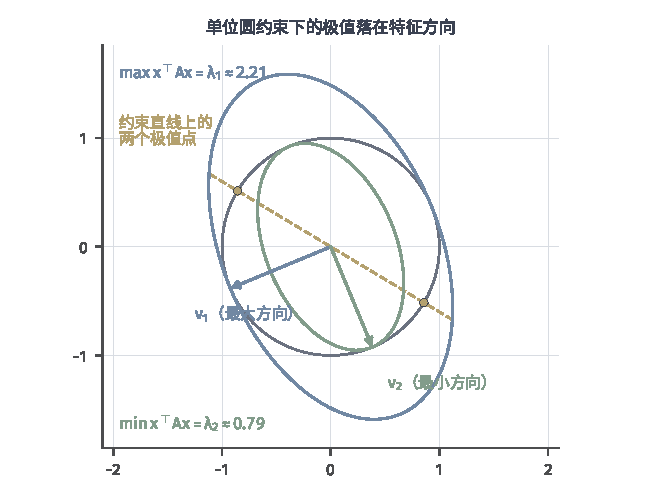
\includegraphics[width=112mm]{figures/00-shared/mathematical-preliminaries-upper/02-linear-spaces/matplotlib/ls-sphere-constrained-extremum/ls-sphere-constrained-extremum.pdf}
  \caption{单位圆约束下的极值落在特征方向。$\bm S=\left[\begin{smallmatrix}2&0.5\\0.5&1\end{smallmatrix}\right]$，
  灰圆为$\lVert\bm x\rVert=1$。蓝椭圆$\bm x^\top\bm S\bm x=\lambda_1\approx2.21$在
  $\pm\bm v_1$处与单位圆相切（最大值），绿椭圆$=\lambda_2\approx0.79$在$\pm\bm v_2$处
  相切（最小值）；黄色虚线为子空间约束直线，其上黄点是该约束下的两个极值。
  $\lambda_{1,2}=(3\pm\sqrt2)/2$。固定复算。}
  \label{fig:ls-sphere-constrained-extremum}
\end{figure}

加权平均介于被平均各数的最小值与最大值之间，由此立即得到两端特征值的极值刻画。
\begin{theorem}[Rayleigh--Ritz]
\label{thm:matrix-analysis-rayleigh-ritz}
\label{eq:matrix-analysis-rayleigh-ritz}
设$\bm S$的特征值为$\lambda_1\geq\cdots\geq\lambda_d$，对应标准正交特征向量$\bm q_1,\ldots,\bm q_d$，则
\begin{equation*}
 \max_{\bm x\neq\bm0}R_{\bm S}(\bm x)=\lambda_1,\qquad
 \min_{\bm x\neq\bm0}R_{\bm S}(\bm x)=\lambda_d,
\end{equation*}
分别在$\bm q_1$与$\bm q_d$取到。
\end{theorem}
\begin{proof}
权重$c_i^2$非负且总和为$1$，所以$\lambda_d\leq\sum_i\lambda_ic_i^2\leq\lambda_1$；取$\bm x=\bm q_1$时只有$c_1=1$，得$\lambda_1$，取$\bm x=\bm q_d$时得$\lambda_d$。
\end{proof}
极值本身唯一，取到极值的方向却未必唯一：$\lambda_1$重复时，其特征空间中每个单位向量都给出最大值；只有在目标特征值单重时，最优方向才唯一（差一个符号）。

\paragraph{齐次最小二乘}
\label{sec:linear-algebra-homogeneous-estimation}

Rayleigh--Ritz定理的一个直接应用是带尺度约束的拟合。有时模型写成$\bm A\bm h\approx\bm0$，只关心$\bm h$各分量之间的比例。这时直接最小化$\lVert\bm A\bm h\rVert_2^2$总会得到平凡解$\bm h=\bm0$，必须先固定尺度。固定$\lVert\bm h\rVert_2=1$后得到的问题称为\term{齐次最小二乘}（homogeneous least squares）：
\begin{equation}
 \min_{\lVert\bm h\rVert_2=1}\ \lVert\bm A\bm h\rVert_2^2
 =\min_{\lVert\bm h\rVert_2=1}\bm h^\top\bm A^\top\bm A\bm h.
 \label{eq:linear-algebra-homogeneous-least-squares}
\end{equation}
右端是对称矩阵$\bm A^\top\bm A$的二次型在单位球面上的最小值。由Rayleigh--Ritz定理，最小值是$\bm A^\top\bm A$的最小特征值，最优$\bm h$是对应的单位特征向量。若$\bm A$有非零零空间，最小值为零，任一单位零空间向量都是最优解。下面的例子属于这种情形。
\begin{example}[一个方程的齐次最小二乘]
\label{ex:ls-homogeneous-least-squares-one-row}
给定一行矩阵$\bm A=[\,1\ -2\,]$。

按式~\eqref{eq:linear-algebra-homogeneous-least-squares}，最优解是$\bm A^\top\bm A$最小特征值的单位特征向量。计算得
\[
 \begin{aligned}
 \bm A^\top\bm A&=\begin{bmatrix}1&-2\\-2&4\end{bmatrix},\\
 \bm A^\top\bm A\,(2,1)^\top&=\bm0,\qquad
 \bm A^\top\bm A\,(1,-2)^\top=5\,(1,-2)^\top .
 \end{aligned}
\]
所以$\bm A^\top\bm A$的特征值为$0$与$5$。

最小特征值$0$对应的单位特征向量为$\bm h=\pm(2,1)^\top/\sqrt5$，它满足$\bm A\bm h=h_1-2h_2=0$。

结论：最小值为$0$，最优解为$\bm h=\pm(2,1)^\top/\sqrt5$；两个符号给出同一个比例$h_1:h_2=2:1$。
\end{example}

\paragraph{Courant--Fischer最小最大原理}

Rayleigh--Ritz定理只刻画两端的特征值。中间的$\lambda_k$不再是整个空间上的极值，但可以借助子空间刻画：在$k$维子空间上取Rayleigh商的最小值，再让子空间变动，取这些最小值中的最大者。

\begin{theorem}[Courant--Fischer]
\label{thm:matrix-analysis-courant-fischer}
\label{eq:matrix-analysis-courant-fischer}
对$k=1,\ldots,d$，
\begin{equation*}
 \lambda_k=\max_{\dim\mathcal V=k}\ \min_{\bm x\in\mathcal V,\bm x\neq\bm0}R_{\bm S}(\bm x)
 =\min_{\dim\mathcal W=d-k+1}\ \max_{\bm x\in\mathcal W,\bm x\neq\bm0}R_{\bm S}(\bm x).
\end{equation*}
\end{theorem}
\begin{proof}
先证第一式。取$\mathcal V_k=\operatorname{span}\{\bm q_1,\dots,\bm q_k\}$，其中单位向量的Rayleigh商是$\lambda_1,\ldots,\lambda_k$的加权平均，不小于$\lambda_k$，所以左端的最大值至少为$\lambda_k$。反过来，任取$k$维子空间$\mathcal V$，令$\mathcal W_k=\operatorname{span}\{\bm q_k,\dots,\bm q_d\}$，它是$d-k+1$维的。由维数公式，
\[
 \dim(\mathcal V\cap\mathcal W_k)\geq\dim\mathcal V+\dim\mathcal W_k-d=1,
\]
所以$\mathcal V$中有非零向量$\bm x$落在$\mathcal W_k$里。它的Rayleigh商是$\lambda_k,\ldots,\lambda_d$的加权平均，不大于$\lambda_k$，因此$\mathcal V$上Rayleigh商的最小值不超过$\lambda_k$。两方面合起来即得第一式。

第二式交换两组特征向量的角色：$\mathcal W_k$上Rayleigh商的最大值恰为$\lambda_k$；任意$d-k+1$维子空间都与$\mathcal V_k$有非零公共向量，其Rayleigh商不小于$\lambda_k$。
\end{proof}
定理只涉及子空间与Rayleigh商，不要求先知道特征向量；第~\ref{sec:ls-spectral-value-sensitivity}节正是用它比较扰动前后的特征值。同样的加权平均论证还可以一次处理$k$个方向，得到前$k$个与后$k$个特征值之和的极值刻画。

\begin{theorem}[迹极值]
\label{thm:matrix-analysis-trace-minimum}
对列标准正交的$\bm V\in\mathbb R^{d\times k}$，
\begin{equation}
 \sum_{i=d-k+1}^{d}\lambda_i\leq\operatorname{tr}(\bm V^\top\bm S\bm V)\leq\sum_{i=1}^{k}\lambda_i,
 \label{eq:matrix-analysis-trace-minimum}
\end{equation}
上下界分别由前$k$个与后$k$个特征向量张成的子空间取到。
\end{theorem}
\begin{proof}
代入$\bm S=\sum_i\lambda_i\bm q_i\bm q_i^\top$，得$\operatorname{tr}(\bm V^\top\bm S\bm V)=\sum_i\lambda_iw_i$，其中$w_i=\lVert\bm V^\top\bm q_i\rVert_2^2$。由$\bm V^\top\bm V=\bm I$得$\lVert\bm V^\top\rVert_2=1$，所以$0\leq w_i\leq1$；又$\sum_iw_i=\lVert\bm V^\top\bm Q\rVert_{\mathrm F}^2=\lVert\bm V\rVert_{\mathrm F}^2=k$。在这两个约束下，
\[
 \begin{aligned}
 \sum_i\lambda_iw_i-\sum_{i\leq k}\lambda_i
 &=\sum_{i\leq k}\lambda_i(w_i-1)+\sum_{i>k}\lambda_iw_i\\
 &\leq\lambda_k\sum_{i\leq k}(w_i-1)+\lambda_k\sum_{i>k}w_i
 =\lambda_k\Bigl(\sum_iw_i-k\Bigr)=0,
 \end{aligned}
\]
其中不等号用到$w_i-1\leq0$、$\lambda_i\geq\lambda_k$（$i\leq k$）与$w_i\geq0$、$\lambda_i\leq\lambda_k$（$i>k$）。这就是上界；对$-\bm S$应用上界即得下界。$\bm V$取前$k$个或后$k$个特征向量时，等号成立。
\end{proof}
上界说明，用$k$维子空间保留二次型的“能量”，最好的选择是前$k$个特征方向，这是主成分分析的代数基础。

\paragraph{广义特征问题}

有时长度不按欧氏范数度量，而按第~\ref{sec:ls-weighted-inner-products}节的加权内积度量，约束$\lVert\bm x\rVert_2=1$相应地换成$\bm x^\top\bm B\bm x=1$（$\bm B\succ0$），要比较的是广义Rayleigh商$\bm x^\top\bm S\bm x/\bm x^\top\bm B\bm x$。它可以化回普通情形。由定理~\ref{thm:ls-gram-factor}写$\bm B=\bm L^\top\bm L$，$\bm L$可逆，令$\bm z=\bm L\bm x$，则$\bm x^\top\bm B\bm x=\bm z^\top\bm z$，而
\[
 \frac{\bm x^\top\bm S\bm x}{\bm x^\top\bm B\bm x}
 =\frac{\bm z^\top\bm L^{-\top}\bm S\bm L^{-1}\bm z}{\bm z^\top\bm z}
\]
是对称矩阵$\bm L^{-\top}\bm S\bm L^{-1}$的普通Rayleigh商。其特征方程$\bm L^{-\top}\bm S\bm L^{-1}\bm z=\mu\bm z$左乘$\bm L^\top$并换回$\bm v=\bm L^{-1}\bm z$，就是下面的方程。
\begin{definition}[广义特征值]
\label{def:matrix-analysis-generalized-eigenvalue}
对实对称$\bm S$与$\bm B\succ0$，称满足
\begin{equation}
 \bm S\bm v=\mu\bm B\bm v,\qquad\bm v\neq\bm0
 \label{eq:matrix-analysis-generalized-eigenproblem}
\end{equation}
的$\mu$为广义特征值，$\bm v$为广义特征向量，求解它们的问题称为\term{广义特征问题}（generalized eigenvalue problem）。
\end{definition}
对$\bm L^{-\top}\bm S\bm L^{-1}$应用谱定理可知：广义特征值全为实数；广义特征向量可以取为$\bm B$正交的，即$\bm v_i^\top\bm B\bm v_j=\delta_{i,j}$（因为$\bm z_i=\bm L\bm v_i$标准正交）；最大、最小广义特征值就是广义Rayleigh商的最大、最小值。

计算时也应走这条换元的路。直接对$\bm B^{-1}\bm S$求特征值虽然得到同样的$\mu$，但$\bm B^{-1}\bm S$一般不对称，会丢掉对称结构带来的正交性与数值稳定性。

\subsection{对称矩阵的函数}
\label{sec:ls-matrix-functions}
\label{sec:matrix-analysis-functions-structured-operations}

多项式$p(\bm S)$可以直接用矩阵的幂与加法算出。平方根、对数、指数这类非多项式函数怎样作用于矩阵？谱定理提示了做法。由$\bm S=\bm Q\bm\Lambda\bm Q^\top$与$\bm Q^\top\bm Q=\bm I$，连乘时相邻的$\bm Q^\top\bm Q$相消，得$\bm S^k=\bm Q\bm\Lambda^k\bm Q^\top$；再按系数相加，得$p(\bm S)=\bm Q\,p(\bm\Lambda)\,\bm Q^\top$。也就是说，多项式在每个特征方向上只作用于对应的特征值。把这一观察作为定义，推广到一般函数。

\paragraph{沿特征方向的定义}

设$\bm S=\bm Q\bm\Lambda\bm Q^\top$，$f$是定义在全部特征值$\lambda_i$上的实函数，令
\begin{equation}
 f(\bm S)=\bm Q\operatorname{diag}\bigl(f(\lambda_1),\ldots,f(\lambda_d)\bigr)\bm Q^\top.
 \label{eq:ls-symmetric-spectral-function}
\end{equation}
$\bm Q$不唯一，需要检查结果是否依赖它的选取。把同一特征值$\lambda$的特征向量归为一组，$\sum_{\lambda_i=\lambda}\bm q_i\bm q_i^\top$是到特征空间$\ker(\bm S-\lambda\bm I)$的正交投影$\bm P_\lambda$，它只依赖这个子空间，与子空间内基的选取无关。于是$f(\bm S)=\sum_\lambda f(\lambda)\bm P_\lambda$，求和遍历不同的特征值，结果由$\bm S$唯一确定。$f(z)=z^k$时，定义回到矩阵幂$\bm S^k$，与已有运算相容。

矩阵函数作用在特征方向上，而不是逐元素作用。下面的例子对照这两种做法。
\begin{example}[矩阵平方根与逐元素开方]
\label{ex:ls-matrix-square-root-two-by-two}
给定示例~\ref{ex:ls-symmetric-spectral-two-by-two}的$\bm S=3\bm q_1\bm q_1^\top+\bm q_2\bm q_2^\top$，取$f(z)=\sqrt z$。按式~\eqref{eq:ls-symmetric-spectral-function}，
\[
 f(\bm S)=\sqrt3\,\bm q_1\bm q_1^\top+\bm q_2\bm q_2^\top
 =\frac12\begin{bmatrix}\sqrt3+1&\sqrt3-1\\\sqrt3-1&\sqrt3+1\end{bmatrix}.
\]
它的平方为
\[
 \frac14\begin{bmatrix}(\sqrt3+1)^2+(\sqrt3-1)^2&2(\sqrt3+1)(\sqrt3-1)\\2(\sqrt3+1)(\sqrt3-1)&(\sqrt3+1)^2+(\sqrt3-1)^2\end{bmatrix}
 =\frac14\begin{bmatrix}8&4\\4&8\end{bmatrix}=\bm S .
\]
逐元素开方得到$\left[\begin{smallmatrix}\sqrt2&1\\1&\sqrt2\end{smallmatrix}\right]$，它的平方是$\left[\begin{smallmatrix}3&2\sqrt2\\2\sqrt2&3\end{smallmatrix}\right]\neq\bm S$。结论：沿特征方向定义的$f(\bm S)$满足$f(\bm S)^2=\bm S$，逐元素开方的结果则不满足。
\end{example}

\paragraph{平方根、实幂与对数}

$\bm S$半正定时，全部$\lambda_i\geq0$，可取$f(z)=\sqrt z$，得到\term{矩阵平方根}（matrix square root）
\[
 \bm S^{1/2}=\bm Q\operatorname{diag}(\sqrt{\lambda_1},\ldots,\sqrt{\lambda_d})\bm Q^\top ,
\]
它半正定且$(\bm S^{1/2})^2=\bm S$。

方程$\bm X^2=\bm S$一般有多个解，例如$\bm I$与$-\bm I$的平方都是$\bm I$；但要求$\bm X$半正定后，解是唯一的。设半正定的$\bm X=\sum_j\mu_j\bm p_j\bm p_j^\top$（$\mu_j\geq0$，$\bm p_j$标准正交）满足$\bm X^2=\bm S$，则$\bm S=\sum_j\mu_j^2\bm p_j\bm p_j^\top$，即每个$\bm p_j$都是$\bm S$的特征向量，特征值为$\mu_j^2$。于是$\bm S$的$\lambda$特征空间恰由满足$\mu_j^2=\lambda$的那些$\bm p_j$张成，而$\mu_j\geq0$迫使这些$\mu_j=\sqrt\lambda$。所以$\bm X$在$\bm S$的每个特征空间上都乘以$\sqrt\lambda$，这正是$\bm S^{1/2}$的作用，$\bm X=\bm S^{1/2}$。

$\bm S$正定时，全部$\lambda_i>0$，还可以取任意实幂$\bm S^\alpha$，例如$\alpha=-1/2$给出逆平方根；也可以取\term{矩阵对数}（matrix logarithm）$\log\bm S=\bm Q\operatorname{diag}(\log\lambda_1,\ldots,\log\lambda_d)\bm Q^\top$。有零特征值时，负幂与对数都没有定义。注意$\log\bm S$是矩阵，而$\log\det\bm S=\sum_i\log\lambda_i=\operatorname{tr}(\log\bm S)$是标量，二者不能混淆。

按定义计算需要完整的谱分解，代价较高。若只需计算$\lVert\bm S^{1/2}\bm x\rVert_2$或作用$\bm S^{-1/2}$做白化，可以用定理~\ref{thm:ls-gram-factor}的因子代替平方根：写$\bm S=\bm L^\top\bm L$，则$\lVert\bm L\bm x\rVert_2^2=\bm x^\top\bm S\bm x=\lVert\bm S^{1/2}\bm x\rVert_2^2$，两者给出同样的长度。第~\ref{chap:linear-equations-and-optimization}章的Cholesky分解把$\bm L$取成三角矩阵，那时作用$\bm L^{-1}$只需解三角方程。

至此，本节的问题有了回答。能用正交矩阵对角化的实矩阵，即具有一组标准正交特征向量的实矩阵，恰好是对称矩阵；谱分解$\bm S=\bm Q\bm\Lambda\bm Q^\top$把它写成沿互相垂直方向的伸缩。特征值同时是Rayleigh商的极值与最小最大值，可以只凭二次型来比较；矩阵函数沿特征方向逐个作用于特征值。但许多重要的方阵并不对称，例如平面旋转与示例~\ref{ex:ls-triangular-power}的上三角矩阵$\left[\begin{smallmatrix}0.8&4\\0&0.5\end{smallmatrix}\right]$。下一节讨论，对一般方阵，坚持用正交矩阵换基时最多能化到多简单。

% 第6章第4节：一般方阵的对角化（复特征值与谱半径、实Schur形与正规矩阵）。

\section{一般方阵的对角化}
\label{sec:ls-general-square-spectrum}

前两节的对角化各有前提：用可逆矩阵对角化，要求有足够多的实特征向量；用正交矩阵对角化，要求矩阵对称。不对称的方阵会在两处偏离这些前提。其一，实特征值可能不够：平面上的$90^\circ$旋转没有实特征向量，第~\ref{sec:ls-matrix-powers}节的对角化在第一步就停止。其二，即使可以对角化，特征向量也可能互不正交：示例~\ref{ex:ls-triangular-power}中矩阵的两条特征方向$(1,0)^\top$与$(-40/3,1)^\top$夹角只有约$4.3^\circ$（计算见示例~\ref{ex:ls-nonnormal-norm-radius}）。本节回答三个问题：非实的特征值在实空间中对应什么作用，怎样用一个数概括矩阵每作用一次的伸缩倍数；若坚持用正交矩阵换基，一般方阵最多能化到多接近对角的形式；什么样的方阵在这种换基下仍能化为分块对角形。

\subsection{复特征值与谱半径}

第~\ref{sec:ls-characteristic-polynomial}节的特征多项式$p_{\bm A}$是$d$次实系数多项式。由代数基本定理，它在复数范围内恰有$d$个根（计重数）。把这些根都称为$\bm A$的特征值，全体特征值组成的集合称为$\bm A$的\term{谱}（spectrum）。由于系数都是实数，若$p_{\bm A}(\lambda)=0$，两边取共轭即得$p_{\bm A}(\bar\lambda)=0$，所以非实根成共轭对出现。实特征值的情形与第~\ref{sec:ls-linear-operators}节相同。

第~\ref{sec:ls-eigen-similarity-invariance}节由系数比较得到$\operatorname{tr}\bm A=\sum_i\lambda_i$与$\det\bm A=\prod_i\lambda_i$，那里要求$p_{\bm A}$能分解为实一次因子。计入复特征值以后，$p_{\bm A}$在复数范围内总能分解为一次因子之积，同样的系数比较说明，这两个等式对每个方阵都成立。

非实特征值在实空间里对应什么作用？设$\lambda=a+\mathrm ib$（$b\neq0$）是特征值。复矩阵$\bm A-\lambda\bm I$的行列式为零，所以有非零的复向量$\bm u+\mathrm i\bm w$满足$\bm A(\bm u+\mathrm i\bm w)=(a+\mathrm ib)(\bm u+\mathrm i\bm w)$，其中$\bm u,\bm w$为实向量。比较两边的实部与虚部，得
\[
 \bm A\bm u=a\bm u-b\bm w,\qquad \bm A\bm w=b\bm u+a\bm w .
\]

这两个等式说明$\operatorname{span}\{\bm u,\bm w\}$在$\bm A$下不变。它是二维的，即$\bm u,\bm w$线性无关。否则$\bm u,\bm w$（不全为零）只张成一条直线$\operatorname{span}\{\bm y\}$，这条直线在$\bm A$下不变，所以$\bm A\bm y=\mu\bm y$，$\mu$为实数；而$\bm u+\mathrm i\bm w$是$\bm y$的复数倍，于是$\bm A(\bm u+\mathrm i\bm w)=\mu(\bm u+\mathrm i\bm w)$，得$\lambda=\mu$为实数，与$b\neq0$矛盾。所以$\operatorname{span}\{\bm u,\bm w\}$是二维实不变子空间。在基$(\bm u,\bm w)$下，$\bm A$的作用由矩阵
\[
 \begin{bmatrix}a&b\\-b&a\end{bmatrix}
 =|\lambda|\begin{bmatrix}\cos\phi&\sin\phi\\-\sin\phi&\cos\phi\end{bmatrix},
 \qquad \cos\phi=\frac{a}{|\lambda|},\ \sin\phi=\frac{b}{|\lambda|}
\]
表示，即$|\lambda|$倍的伸缩加一次旋转。

所以无论特征值是实是复，它的模长$|\lambda|$都是沿相应方向或平面每作用一次的伸缩倍数；复特征值的情形在基$(\bm u,\bm w)$的坐标中度量。全部特征值模长的最大值
\[
 \rho(\bm A)=\max_i|\lambda_i(\bm A)|
\]
称为\term{谱半径}（spectral radius）。例如$90^\circ$旋转的特征值为$\pm\mathrm i$，谱半径为$1$：它不改变长度，只改变方向。

\subsection{实Schur形与正规矩阵}

\paragraph{实Schur形}

一般方阵未必能对角化，更未必能用正交矩阵对角化。退一步，能否用正交矩阵把它化为上三角形？上三角形同样便于计算：对角元就是特征值，解方程和求幂都可以从最后一个坐标逐个向前推。实特征值不够时，实上三角形不可能存在，因为它的对角元就是特征值，必须全是实数；但允许对角线上出现$2\times2$块以后，答案总是肯定的。

\begin{theorem}[实Schur形]
\label{thm:ls-real-schur}
对任意$\bm A\in\mathbb R^{d\times d}$，存在正交矩阵$\bm Q$与分块上三角矩阵$\bm T$，使
\begin{equation}
 \bm A=\bm Q\bm T\bm Q^{\top},
 \label{eq:matrix-analysis-schur-decomposition}
\end{equation}
$\bm T$的对角块为$1\times1$（实特征值）或$2\times2$（一对共轭特征值），对角块下方全为零。$\bm A$的特征值就是各对角块的特征值。
\end{theorem}
\begin{proof}
对$d$归纳，思路与谱定理相同：先找一个不变子空间，再对其正交补降维。若$\bm A$有实特征值$\lambda$，取单位特征向量$\bm q_1$并扩充为正交矩阵$\bm Q_1=[\bm q_1,\bm Q_2]$。由$\bm A\bm q_1=\lambda\bm q_1$与$\bm Q_2^\top\bm q_1=\bm0$，$\bm Q_1^\top\bm A\bm Q_1$的第一列为$\lambda\bm e_1$，即
\[
 \bm Q_1^\top\bm A\bm Q_1=\begin{bmatrix}\lambda&*\\\bm0&\bm Q_2^\top\bm A\bm Q_2\end{bmatrix}.
\]
若没有实特征值，取上一小节得到的二维不变子空间，用它的一组标准正交基$\bm q_1,\bm q_2$同样扩充，得到左上角为$2\times2$块、其下方为零的分块形式，该块的特征值是$\lambda,\bar\lambda$。分块上三角矩阵的特征多项式是对角块特征多项式之积，所以右下块的特征值恰为其余特征值。对右下块应用归纳假设，再把两次正交变换合并，即得结论。
\end{proof}
实际计算先用Householder反射化为上Hessenberg形，再作带位移的QR迭代，标准数值软件都提供这一分解；本卷只使用它的存在性。第~\ref{sec:ls-sylvester-schur}节求解Sylvester方程时，用的正是这一形式。

\paragraph{正规矩阵}

Schur形什么时候是分块对角的？实对称矩阵是一例。这时$\bm T=\bm Q^\top\bm A\bm Q$仍对称，它的$2\times2$对角块也对称，特征值为实数，不可能对应一对共轭特征值，所以$\bm T$只有$1\times1$对角块，是上三角矩阵；对称的上三角矩阵只能是对角矩阵，这又一次得到谱定理。更一般地，第~\ref{sec:ls-adjoints}节把满足$TT^\star=T^\star T$的算子称为正规算子。在标准坐标下伴随就是转置，满足$\bm A^\top\bm A=\bm A\bm A^\top$的矩阵称为\term{正规矩阵}（normal matrix）；对称、反对称与正交矩阵都是正规的。

正规矩阵的Schur形$\bm T$分块对角。首先$\bm T$也正规：$\bm T^\top\bm T=\bm Q^\top\bm A^\top\bm A\bm Q=\bm Q^\top\bm A\bm A^\top\bm Q=\bm T\bm T^\top$。比较$\bm T^\top\bm T$与$\bm T\bm T^\top$的左上角对角块：前者是$\bm T_{1,1}^\top\bm T_{1,1}$，因为$\bm T$的第一块列只有$\bm T_{1,1}$非零；后者是$\sum_j\bm T_{1,j}\bm T_{1,j}^\top$。两边取迹，得
\[
 \lVert\bm T_{1,1}\rVert_{\mathrm F}^2=\lVert\bm T_{1,1}\rVert_{\mathrm F}^2+\sum_{j>1}\lVert\bm T_{1,j}\rVert_{\mathrm F}^2 ,
\]
故第一块行的非对角块全为零。去掉第一块后，剩下的矩阵仍正规，逐块推下去可知$\bm T$分块对角。

每个$2\times2$对角块$\left[\begin{smallmatrix}p&q\\r&s\end{smallmatrix}\right]$也正规。比较两边的$(1,1)$元得$q^2=r^2$。若$q=r$，块对称，特征值为实数，与$2\times2$块对应一对共轭特征值矛盾；所以$r=-q\neq0$。再比较$(1,2)$元得$2q(s-p)=0$，即$s=p$。于是每块都形如$\left[\begin{smallmatrix}a&b\\-b&a\end{smallmatrix}\right]$，是模长乘旋转。反过来，若正交矩阵$\bm Q$把$\bm A$化为分块对角矩阵$\bm T$，且每块是一个数或这种模长乘旋转的块，则每块与自己的转置可交换，$\bm T^\top\bm T=\bm T\bm T^\top$，从而$\bm A=\bm Q\bm T\bm Q^\top$正规。所以正规矩阵恰好是能用标准正交基化为这种分块对角形的实方阵。

总之，正规矩阵沿一组标准正交的方向或平面只作伸缩，或伸缩加旋转。$\bm T^k$仍分块对角，每块是$\lambda^k$或$|\lambda|^k$乘一个旋转，二范数为$|\lambda|^k$；正交变换又不改变谱范数，所以$\lVert\bm A^k\rVert_2=\lVert\bm T^k\rVert_2=\max_i|\lambda_i|^k=\rho(\bm A)^k$。也就是说，正规矩阵每一步的最大放大倍数恰好就是谱半径。

\paragraph{非正规矩阵}
由上一段，非正规矩阵的Schur形$\bm T$不可能是由数与模长乘旋转块组成的分块对角形：它要么含非零的非对角块，要么某个$2\times2$对角块本身不正规。非正规矩阵也不能用一组标准正交的特征向量对角化，否则它对称。这时矩阵范数可以远大于谱半径，下面的例子显示了这种分离。
\begin{example}[非正规矩阵的范数与谱半径]
\label{ex:ls-nonnormal-norm-radius}
给定示例~\ref{ex:ls-triangular-power}的$\bm A=\left[\begin{smallmatrix}0.8&4\\0&0.5\end{smallmatrix}\right]$，比较它的谱半径、一步的放大倍数与特征方向的夹角。

它不正规：$\bm A^\top\bm A$的$(1,1)$元为$0.8^2=0.64$，$\bm A\bm A^\top$的$(1,1)$元为$0.8^2+4^2=16.64$。特征值为$0.8$与$0.5$，所以$\rho(\bm A)=0.8$。一步作用把$(0,1)^\top$送到$(4,0.5)^\top$，长度为$\sqrt{16.25}>4$，所以$\lVert\bm A\rVert_2>4$。两条特征方向$\bm v_1=(1,0)^\top$与$\bm v_2=(-40/3,1)^\top$的夹角$\theta$满足
\[
 \cos\theta=\frac{|\bm v_1^\top\bm v_2|}{\lVert\bm v_1\rVert_2\lVert\bm v_2\rVert_2}
 =\frac{40/3}{\sqrt{(40/3)^2+1}}\approx0.997,
\]
即$\theta\approx4.3^\circ$。结论：两条特征方向几乎平行，一步的最大放大倍数超过$4$，而谱半径只有$0.8$。
\end{example}
谱半径描述反复作用的长期倍率，范数描述一步的最大放大；非正规时二者分离。第~\ref{sec:ls-matrix-power-behavior}节将看到，这会造成先放大、后衰减的瞬态。

至此，本节的问题有了回答。实矩阵的特征值可能是复数，一对共轭特征值$a\pm\mathrm ib$对应一个二维不变平面上的伸缩加旋转；谱半径$\rho(\bm A)$概括每作用一次的长期伸缩倍数。坚持用标准正交基时，一般方阵只能化为实Schur形；恰好能化为由数与模长乘旋转块组成的分块对角形的是正规矩阵，它每一步的最大放大等于谱半径，非正规矩阵的范数与谱半径则可能相差悬殊。这些结论都要求矩阵把空间映到自身，并且输入、输出用同一组基。若允许两端各取一组标准正交基，这一限制就消失了：下一节说明，任何矩阵都能这样化为对角形。

% 第6章第5节：奇异值分解（构造、奇异值与矩阵范数、极分解、最佳低秩逼近）。

\section{奇异值分解}
\label{sec:ls-svd}

前面几节都让输入与输出使用同一组基。在这一要求下用标准正交基换基，只有对称矩阵能化为实对角形，正规矩阵能化为分块对角形，一般方阵只能化为分块上三角的实Schur形。矩形矩阵$\bm A\in\mathbb R^{m\times d}$的输入在$\mathbb R^d$中、输出在$\mathbb R^m$中，“同一组基”与特征向量都无从谈起。于是放宽要求：能否在输入端找一组标准正交方向$\bm v_i$，在输出端找一组标准正交方向$\bm u_i$，使
\[
 \bm A\bm v_i=\sigma_i\bm u_i ,\qquad \sigma_i\geq0,
\]
即$\bm A$只把第$i$个输入方向伸缩$\sigma_i$倍后送到第$i$个输出方向？本节先证明这对任意矩阵都可以做到。所需的方向来自对称矩阵$\bm A^\top\bm A$的特征方向，构造只用到谱定理（定理~\ref{thm:ls-real-symmetric-spectral}）。然后说明这种分解给出了什么：谱范数与Frobenius范数的值，把方阵的作用分成伸缩与转动的极分解，以及给定秩上限时最好的近似。

\subsection{SVD的构造}

先看这样的方向若存在，应当是什么。设$\bm x=\sum_ic_i\bm v_i$，则$\bm A\bm x=\sum_ic_i\sigma_i\bm u_i$，由$\bm u_i$标准正交，
\[
 \bm x^\top\bm A^\top\bm A\bm x=\lVert\bm A\bm x\rVert_2^2=\sum_i\sigma_i^2c_i^2 .
\]
与二次型展开式~\eqref{eq:matrix-analysis-quadratic-spectral-form}比较可知，$\bm v_i$应是对称矩阵$\bm A^\top\bm A$的特征向量，$\sigma_i^2$是对应的特征值。这提示从$\bm A^\top\bm A$出发构造。

令$\bm S=\bm A^\top\bm A$。它对称，而且半正定：$\bm x^\top\bm A^\top\bm A\bm x=\lVert\bm A\bm x\rVert_2^2\geq0$。由谱定理，存在$\mathbb R^d$的标准正交基$\bm v_1,\ldots,\bm v_d$使$\bm A^\top\bm A\bm v_i=\lambda_i\bm v_i$，且$\lambda_1\geq\cdots\geq\lambda_d\geq0$。设前$r$个特征值为正，记$\sigma_i=\sqrt{\lambda_i}>0$（$i\leq r$）。其余的$\bm v_j$满足$\lVert\bm A\bm v_j\rVert_2^2=\bm v_j^\top\bm A^\top\bm A\bm v_j=0$，即$\bm A\bm v_j=\bm0$。

对$i\leq r$定义输出方向$\bm u_i=\bm A\bm v_i/\sigma_i$。它们标准正交：
\[
 \bm u_i^\top\bm u_j
 =\frac{\bm v_i^\top\bm A^\top\bm A\bm v_j}{\sigma_i\sigma_j}
 =\frac{\sigma_j^2\,\bm v_i^\top\bm v_j}{\sigma_i\sigma_j}=\delta_{i,j}.
\]
再把$\bm u_1,\dots,\bm u_r$扩充为$\mathbb R^m$的标准正交基$\bm u_1,\ldots,\bm u_m$。

现在把任意$\bm x$展开为$\bm x=\sum_i(\bm v_i^\top\bm x)\bm v_i$，再利用$\bm A\bm v_i=\sigma_i\bm u_i$（$i\leq r$）与$\bm A\bm v_j=\bm0$（$j>r$），得
\[
 \bm A\bm x=\sum_{i=1}^r\sigma_i\bm u_i(\bm v_i^\top\bm x).
\]
这对所有$\bm x$成立，所以$\bm A$是$r$个秩一矩阵之和：
\begin{equation}
 \bm A=\sum_{i=1}^r\sigma_i\bm u_i\bm v_i^\top.
 \label{eq:matrix-analysis-svd-rank-one-sum}
\end{equation}
由这个和式，$\operatorname{range}(\bm A)$由$\bm u_1,\ldots,\bm u_r$张成；又因为$\bm u_i$线性无关且$\sigma_i>0$，$\bm A\bm x=\bm0$当且仅当$\bm v_i^\top\bm x=0$（$i\leq r$），所以$\ker\bm A$由$\bm v_{r+1},\ldots,\bm v_d$张成。于是$r=\operatorname{rank}\bm A$。把这些向量排成矩阵，就得到下面的结论。

\begin{theorem}[SVD的存在]
\label{thm:ls-svd-existence}
对任意$\bm A\in\mathbb R^{m\times d}$，存在正交矩阵$\bm U\in\mathbb R^{m\times m}$、$\bm V\in\mathbb R^{d\times d}$与对角矩阵$\bm\Sigma\in\mathbb R^{m\times d}$，使$\bm A=\bm U\bm\Sigma\bm V^\top$；$\bm\Sigma$的对角元$\sigma_1\geq\cdots\geq\sigma_{\min(m,d)}\geq0$，其中恰有$\operatorname{rank}\bm A$个为正。
\end{theorem}

\begin{definition}[奇异值分解]
\label{def:matrix-analysis-svd}
称
\begin{equation}
 \bm A=\bm U\bm\Sigma\bm V^\top
 \label{eq:matrix-analysis-svd}
\end{equation}
为$\bm A$的\term{奇异值分解}（singular value decomposition, SVD），$\bm\Sigma$的对角元$\sigma_i$称为\term{奇异值}（singular value），$\bm U$、$\bm V$的列$\bm u_i$、$\bm v_i$分别称为左、右\term{奇异向量}（singular vector）。
\end{definition}

图~\ref{fig:ls-svd-construction}把构造拆成三步：形成$\bm A^\top\bm A$；由谱定理将其对角化；开方得到奇异值，再由$\bm u_i=\bm A\bm v_i/\sigma_i$得到左奇异向量。

\begin{figure*}[htbp]
  \centering
  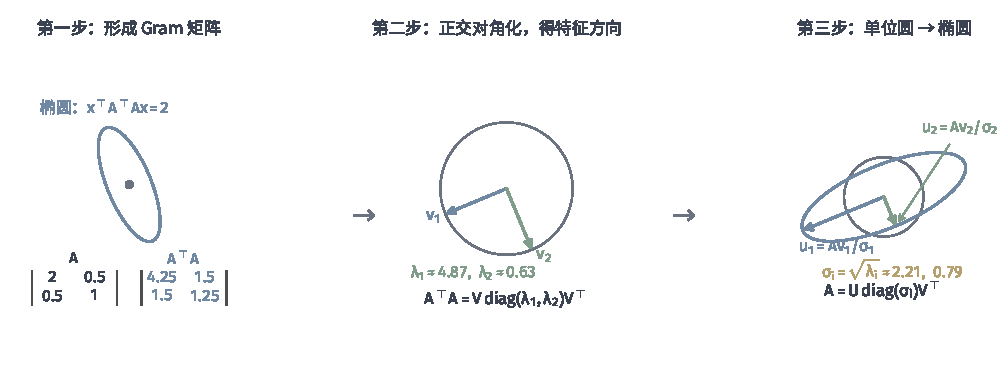
\includegraphics[width=168.998mm]{figures/00-shared/mathematical-preliminaries-upper/02-linear-spaces/matplotlib/ls-svd-construction/ls-svd-construction.pdf}
  \caption{SVD 构造三部曲。以$\bm A=\left[\begin{smallmatrix}2&0.5\\0.5&1\end{smallmatrix}\right]$为例：
  (1)形成$\bm A^\top\bm A=\left[\begin{smallmatrix}4.25&1.5\\1.5&1.25\end{smallmatrix}\right]$；
  (2)由谱定理对角化，特征值$\lambda_1\approx4.87,\lambda_2\approx0.63$；
  (3)$\sigma_i=\sqrt{\lambda_i}\approx2.21,0.79$，右奇异向量$\bm v_i$即特征向量，
  左奇异向量$\bm u_i=\bm A\bm v_i/\sigma_i$。解析式教学构造。}
  \label{fig:ls-svd-construction}
\end{figure*}

几何上，$\bm A$把输入端的单位球面映成输出端的椭球面（秩亏时椭球退化）：$\bm v_i$方向的单位向量被送到长度为$\sigma_i$的半轴$\sigma_i\bm u_i$。图~\ref{fig:matrix-analysis-svd-geometry}用二维旋转矩阵$\bm R(\theta)=\left[\begin{smallmatrix}\cos\theta&-\sin\theta\\\sin\theta&\cos\theta\end{smallmatrix}\right]$构造了一个输入方向与输出方向不同的例子。

\begin{figure*}[htbp]
  \centering
  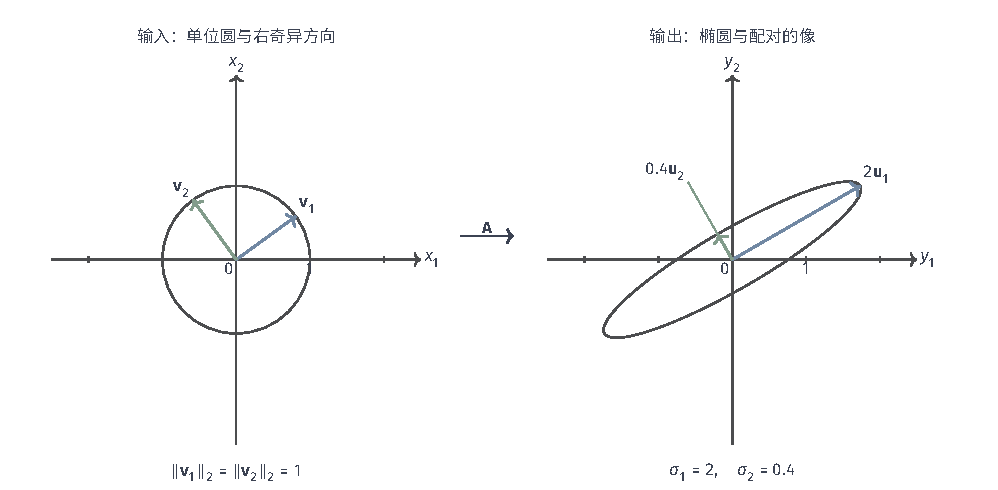
\includegraphics[width=168.998mm]{figures/00-shared/mathematical-preliminaries-upper/02-linear-spaces/tikz/matrix-analysis-svd-geometry/figure.pdf}
  \caption{矩阵$\bm A=\bm R(\pi/6)\operatorname{diag}(2,0.4)\bm R(\pi/5)^\top$
  将单位圆变为椭圆。蓝、绿分别对应两个奇异方向；同色箭头在左侧标出$\bm v_i$，
  在右侧标出其像$\sigma_i\bm u_i$。两侧坐标比例相同。奇异值决定长度变化，左右方向可以不同，
  因而这不是沿特征方向的同空间缩放。图为教学构造。}
  \label{fig:matrix-analysis-svd-geometry}
\end{figure*}

奇异值由$\bm A$唯一确定，它们是$\bm A^\top\bm A$特征值的平方根。奇异向量则不唯一：$\sigma_i$重复时，对应子空间内的任意标准正交基都可以使用；单个$\sigma_i$的一对$\bm u_i,\bm v_i$也可以同时变号。

构造虽然从$\bm A^\top\bm A$出发，数值计算却并不真的形成它：$\bm A^\top\bm A$的特征值是$\sigma_i^2$，小奇异值平方后更小，在舍入中最先失去精度，第~\ref{chap:linear-equations-and-optimization}章讨论最小二乘的数值敏感性时会具体看到这一点。标准算法直接对$\bm A$从两侧施加正交变换，把它化为上双对角形，再迭代求出奇异值；只需要前几个奇异方向时，可以只计算相应的部分。

\subsection{奇异值与矩阵范数}

第~\ref{sec:ls-frobenius-norm}节与第~\ref{sec:ls-matrix-norms}节分别定义了Frobenius范数与谱范数，但没有给出谱范数的算法。SVD直接给出两者的值。对$\bm x=\sum_ic_i\bm v_i$，
\[
 \lVert\bm A\bm x\rVert_2^2=\sum_{i\leq r}\sigma_i^2c_i^2\leq\sigma_1^2\sum_ic_i^2=\sigma_1^2\lVert\bm x\rVert_2^2 ,
\]
等号在$\bm x=\bm v_1$时成立；而$\lVert\bm A\rVert_{\mathrm F}^2=\operatorname{tr}(\bm A^\top\bm A)$等于$\bm A^\top\bm A$的特征值之和$\sum_i\sigma_i^2$。因此
\begin{align}
 \lVert\bm A\rVert_2&=\sigma_1,
 \label{eq:matrix-analysis-spectral-norm}\\
 \lVert\bm A\rVert_{\mathrm F}&=\Bigl(\sum_{i=1}^r\sigma_i^2\Bigr)^{1/2}.
 \label{eq:matrix-analysis-frobenius-norm}
\end{align}
同一展开也给出最弱的放大。$d\leq m$时$\lVert\bm A\bm x\rVert_2\geq\sigma_d\lVert\bm x\rVert_2$，等号在$\bm x=\bm v_d$时成立，秩亏时$\sigma_d=0$。对可逆方阵，$\bm A^{-1}=\sum_i\sigma_i^{-1}\bm v_i\bm u_i^\top$（直接相乘可验证$\bm A\bm A^{-1}=\sum_i\bm u_i\bm u_i^\top=\bm I$），它的最大奇异值是$1/\sigma_d$，所以$\lVert\bm A^{-1}\rVert_2=1/\sigma_d$。

最大奇异值衡量最强的放大，最小奇异值衡量最弱的放大，二者之比就是第~\ref{sec:ls-perturbation-conditioning}节的条件数。齐次最小二乘~\eqref{eq:linear-algebra-homogeneous-least-squares}的最优解也可以由此读出：它是$\bm V$的最后一列$\bm v_d$，因为按构造，$\bm v_d$是$\bm A^\top\bm A$最小特征值的单位特征向量。

\subsection{极分解}

SVD还可以把方阵的作用分成“伸缩”与“转动”两步，类似于把复数写成模长与单位复数之积。设$\bm A\in\mathbb R^{d\times d}$有SVD$\bm A=\bm U\bm\Sigma\bm V^\top$，在$\bm U$与$\bm\Sigma$之间插入$\bm V^\top\bm V=\bm I$，得$\bm A=(\bm U\bm V^\top)(\bm V\bm\Sigma\bm V^\top)$。
\begin{definition}[极分解]
\label{def:matrix-analysis-polar-decomposition}
方阵$\bm A$的\term{极分解}（polar decomposition）是
\begin{equation}
 \bm A=\bm W\bm H,\qquad \bm W=\bm U\bm V^\top,\quad \bm H=\bm V\bm\Sigma\bm V^\top=(\bm A^\top\bm A)^{1/2},
 \label{eq:matrix-analysis-polar-decomposition}
\end{equation}
其中$\bm W$正交，$\bm H$对称半正定。
\end{definition}
$\bm H$先沿$\bm v_i$方向伸缩，$\bm W$再作正交变换。由$\bm H^2=\bm V\bm\Sigma^2\bm V^\top=\bm A^\top\bm A$及半正定平方根的唯一性，$\bm H$由$\bm A$唯一确定；$\bm A$可逆时$\bm H$可逆，$\bm W=\bm A\bm H^{-1}$也唯一。

正交因子$\bm W$是Frobenius范数下离$\bm A$最近的正交矩阵。对正交$\bm Z$，$\lVert\bm Z\rVert_{\mathrm F}^2=d$，展开得$\lVert\bm A-\bm Z\rVert_{\mathrm F}^2=\lVert\bm A\rVert_{\mathrm F}^2+d-2\operatorname{tr}(\bm Z^\top\bm A)$，所以只需让$\operatorname{tr}(\bm Z^\top\bm A)$最大。由迹的循环性，
\[
 \operatorname{tr}(\bm Z^\top\bm U\bm\Sigma\bm V^\top)=\operatorname{tr}(\bm V^\top\bm Z^\top\bm U\,\bm\Sigma)=\sum_i\sigma_i(\bm V^\top\bm Z^\top\bm U)_{i,i}.
\]
$\bm V^\top\bm Z^\top\bm U$是正交矩阵，其列是单位向量，对角元不超过$1$，故迹不超过$\sum_i\sigma_i$；取$\bm Z=\bm U\bm V^\top$时该矩阵为$\bm I$，等号成立。含噪的旋转估计常用这一步把近似正交的矩阵修正为正交矩阵。

\subsection{最佳低秩逼近}
\label{sec:ls-low-rank-solve}
\label{sec:ls-full-svd-solve}
\label{sec:matrix-analysis-svd-low-rank}

数据矩阵常常近似低秩：少数几个方向承载了大部分信息。给定秩上限$k$，怎样找离$\bm A$最近的秩不超过$k$的矩阵？秩一分解~\eqref{eq:matrix-analysis-svd-rank-one-sum}把$\bm A$按奇异值从大到小拆成$r$项，一个自然的候选是只保留前$k$项。

设$\bm A\in\mathbb R^{m\times d}$的非零奇异值为$\sigma_1\geq\cdots\geq\sigma_r>0$，称
\begin{equation}
 \bm A_k=\sum_{i=1}^k\sigma_i\bm u_i\bm v_i^\top,
 \qquad 0\leq k<r
 \label{eq:matrix-analysis-truncated-svd}
\end{equation}
为\term{截断SVD}（truncated SVD），$k=0$时$\bm A_0=\bm0$。

余下的$\bm A-\bm A_k=\sum_{i>k}\sigma_i\bm u_i\bm v_i^\top$本身就是一个SVD，最大奇异值为$\sigma_{k+1}$，由式~\eqref{eq:matrix-analysis-spectral-norm}与式~\eqref{eq:matrix-analysis-frobenius-norm}直接读出两种误差：
\begin{equation}
 \lVert\bm A-\bm A_k\rVert_2=\sigma_{k+1},\qquad
 \lVert\bm A-\bm A_k\rVert_{\mathrm F}
 =\Bigl(\sum_{i=k+1}^r\sigma_i^2\Bigr)^{1/2}.
 \label{eq:ls-truncated-errors}
\end{equation}
谱范数误差是最坏单位输入的输出偏差，Frobenius误差累计全部元素的平方偏差。下面的定理说明，在这两种范数下没有比截断SVD更好的秩$k$近似。

\begin{theorem}[Eckart--Young--Mirsky最佳低秩逼近]
\label{thm:ls-best-low-rank}
\label{thm:matrix-analysis-best-low-rank}
对$0\leq k<r=\operatorname{rank}\bm A$，
\begin{align}
 \min_{\operatorname{rank}\bm B\leq k}\lVert\bm A-\bm B\rVert_2
 &=\sigma_{k+1},
 \label{eq:matrix-analysis-best-rank-k-spectral}\\
 \min_{\operatorname{rank}\bm B\leq k}\lVert\bm A-\bm B\rVert_{\mathrm F}
 &=\Bigl(\sum_{i=k+1}^r\sigma_i^2\Bigr)^{1/2},
 \label{eq:matrix-analysis-best-rank-k-frobenius}
\end{align}
两个最小值都由截断SVD$\bm A_k$达到。
\end{theorem}
\begin{proof}
式~\eqref{eq:ls-truncated-errors}说明$\bm A_k$达到右端，只需证明任意秩不超过$k$的$\bm B$误差都不更小。$k=0$时$\bm B=\bm0$，结论即式~\eqref{eq:ls-truncated-errors}，下设$k\geq1$。

谱范数情形。$\ker\bm B$的维数至少为$d-k$，子空间$\operatorname{span}\{\bm v_1,\ldots,\bm v_{k+1}\}$的维数为$k+1$，两者维数之和超过$d$，必有公共单位向量$\bm x=\sum_{i=1}^{k+1}c_i\bm v_i$，$\sum_ic_i^2=1$。由$\bm B\bm x=\bm0$，
\begin{equation}
 \lVert(\bm A-\bm B)\bm x\rVert_2
 =\lVert\bm A\bm x\rVert_2
 =\Bigl(\sum_{i=1}^{k+1}\sigma_i^2c_i^2\Bigr)^{1/2}
 \geq\sigma_{k+1},
 \label{eq:ls-spectral-lower-bound}
\end{equation}
所以$\lVert\bm A-\bm B\rVert_2\geq\sigma_{k+1}$。

Frobenius情形。正交变换不改变Frobenius范数，令$\bm C=\bm U^\top\bm B\bm V$，则$\operatorname{rank}\bm C=\operatorname{rank}\bm B\leq k$，且$\lVert\bm A-\bm B\rVert_{\mathrm F}=\lVert\bm\Sigma-\bm C\rVert_{\mathrm F}$。设$\bm P$为到$\bm C$列空间的正交投影，则$\operatorname{tr}\bm P=\operatorname{rank}\bm C\leq k$，且$\bm P\bm C=\bm C$。把$\bm\Sigma-\bm C$拆成$(\bm I-\bm P)\bm\Sigma$与$\bm P\bm\Sigma-\bm C$，两部分的每一列分别落在互相正交的子空间中，于是
\[
 \lVert\bm\Sigma-\bm C\rVert_{\mathrm F}^2
 =\lVert(\bm I-\bm P)\bm\Sigma\rVert_{\mathrm F}^2+\lVert\bm P\bm\Sigma-\bm C\rVert_{\mathrm F}^2
 \geq\lVert\bm\Sigma\rVert_{\mathrm F}^2-\lVert\bm P\bm\Sigma\rVert_{\mathrm F}^2 .
\]
$\bm\Sigma$的第$i$列是$\sigma_i\bm e_i$，所以保留部分为$\lVert\bm P\bm\Sigma\rVert_{\mathrm F}^2=\sum_i\sigma_i^2w_i$，其中$w_i=\lVert\bm P\bm e_i\rVert_2^2\in[0,1]$，且$\sum_iw_i\leq\lVert\bm P\rVert_{\mathrm F}^2=\operatorname{tr}\bm P\leq k$。与迹极值定理的证明相同，由$\sigma_i$降序，
\[
 \sum_i\sigma_i^2w_i-\sum_{i\leq k}\sigma_i^2
 =\sum_{i\leq k}\sigma_i^2(w_i-1)+\sum_{i>k}\sigma_i^2w_i
 \leq\sigma_k^2\Bigl(\sum_iw_i-k\Bigr)\leq0 .
\]
即保留部分不超过$\sum_{i\leq k}\sigma_i^2$，误差平方至少为$\lVert\bm\Sigma\rVert_{\mathrm F}^2-\sum_{i\leq k}\sigma_i^2=\sum_{i>k}\sigma_i^2$。
\end{proof}
这一结论最早由Eckart与Young给出\scite{eckart1936}。上面的证明只处理谱范数与Frobenius范数；误差改用加权、逐元素或分组的度量时，最优性需要重新论证，截断SVD一般不再是最优解。图~\ref{fig:ls-low-rank-truncation}画出截断的几何：单位圆经$\bm A$变成椭圆，秩一近似把椭圆压成主轴方向的线段，残留误差恰为舍弃的$\sigma_2$。

\begin{figure*}[htbp]
  \centering
  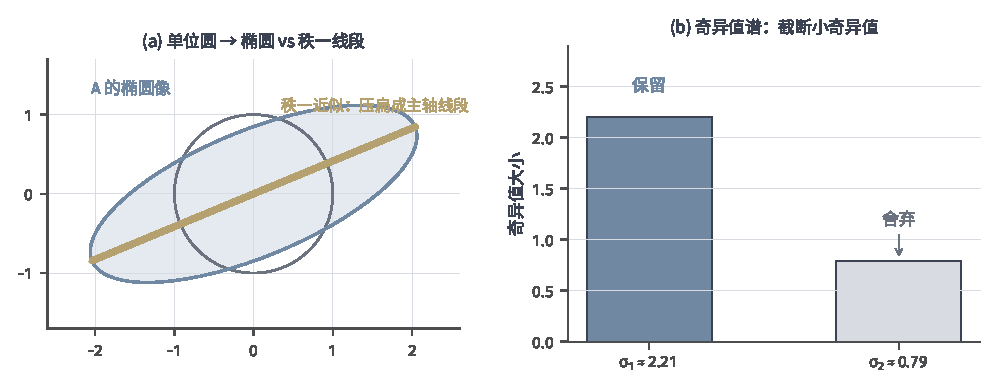
\includegraphics[width=168.998mm]{figures/00-shared/mathematical-preliminaries-upper/02-linear-spaces/matplotlib/ls-low-rank-truncation/ls-low-rank-truncation.pdf}
  \caption{低秩截断的几何。$\bm A=\left[\begin{smallmatrix}2&0.5\\0.5&1\end{smallmatrix}\right]$，
  灰圆为单位圆，蓝椭圆为$\bm A$的像。左：黄粗线段为秩一近似$\bm A_1=\sigma_1\bm v_1\bm v_1^\top$
  的像，椭圆被压成长$2\sigma_1$的线段；右：$\sigma_1\approx2.21$（保留）、$\sigma_2\approx0.79$
  （舍弃），算子范数误差$\lVert\bm A-\bm A_1\rVert_2=\sigma_2$。$\sigma_{1,2}=(3\pm\sqrt2)/2$。
  固定复算。}
  \label{fig:ls-low-rank-truncation}
\end{figure*}

回到本节开头的问题：任意矩阵都能写成$\bm A=\sum_{i\leq r}\sigma_i\bm u_i\bm v_i^\top$，在输入、输出两侧各取一组标准正交方向后，它只是逐个方向的伸缩。奇异值由$\bm A$唯一确定，最大奇异值是谱范数，平方和是Frobenius范数的平方，最小奇异值衡量最弱的放大；方阵还可以写成正交因子与半正定因子之积；按奇异值从大到小截断，得到谱范数与Frobenius范数下的最佳低秩逼近。同一个和式还能反过来用：把每一项$\sigma_i\bm u_i\bm v_i^\top$换成$\sigma_i^{-1}\bm v_i\bm u_i^\top$，就得到秩亏、不相容方程的最小范数最小二乘解，这一构造留到第~\ref{chap:linear-equations-and-optimization}章与线性方程的求解一起讨论。

到这里，本章的第一个问题告一段落：由特征向量组成的基（若存在）使算子的矩阵成为对角形；要求基标准正交时，对称矩阵仍能对角化，一般方阵只能化为实Schur形；输入、输出各取一组标准正交基时，任意矩阵都能对角化。后面三节用这些最简形式研究线性作用的性质，首先是一次作用对误差的放大。最强与最弱的放大分别由最大与最小奇异值给出，下一节用它们定义条件数。

% 第6章第6节：条件数（输入、输出与误差，条件数的定义，基本运算的敏感度）。

\section{条件数}
\label{sec:ls-perturbation}
\label{sec:linear-algebra-stability}
\label{sec:matrix-analysis-conditioning-perturbation}

前五节为线性作用找到了最简形式。从本节起，用这些形式研究线性作用的性质，首先是它对误差的反应。实际交给计算的数据总带误差：测量有噪声，记录有截断，上一步计算有舍入。数据与理想输入相差一点时，答案相差多少？允许范围内的输入增量称为\term{扰动}（perturbation）。扰动分析不改变任务本身，只测量输入的增量在输出中被放大多少倍。

本节先确定怎样度量输入与输出的误差，再定义衡量最坏放大倍数的条件数，说明矩阵的条件数就是最大与最小奇异值之比，最后用同样的增量展开检查几种基本运算。线性方程与最小二乘的解对数据的敏感度，要等第~\ref{chap:linear-equations-and-optimization}章建立求解方法之后，再用本节的工具讨论。

\subsection{输入、输出与误差}

为了统一讨论，把任务看作映射$F$：理想输入$\bm z$对应输出$F(\bm z)$，实际输入为$\bm z+\Delta\bm z$，输出增量为
\[
 \Delta\bm y=F(\bm z+\Delta\bm z)-F(\bm z).
\]
任务不同，比较的输出也不同：矩阵乘向量比较输出向量，求逆比较逆矩阵，解方程比较解向量，谱分解要分别比较特征值与特征子空间。这里只改变数据，不更换算法；算法在机器上产生的舍入误差是另一个来源，第~\ref{chap:linear-equations-and-optimization}章讨论线性方程的数值敏感性时再单独处理。

衡量增量大小有两种方式。\term{绝对误差}（absolute error）直接取增量的范数$\lVert\Delta\bm z\rVert$、$\lVert\Delta\bm y\rVert$。当输入与输出本身有尺度时，更常用\term{相对误差}（relative error）
\[
 \frac{\lVert\Delta\bm z\rVert}{\lVert\bm z\rVert},
 \qquad
 \frac{\lVert\Delta\bm y\rVert}{\lVert F(\bm z)\rVert}.
\]
相对误差在整体缩放下不变，反映变化占原有量的比例；但输出接近零时它失去意义，应改报绝对误差。

误差读数还依赖范数与允许改变的分量：只改右端、同时改矩阵与右端、要求扰动保持对称，是三个不同的扰动问题，敏感度一般不同。

\subsection{条件数的定义}
\label{sec:ls-perturbation-conditioning}

输入增量可以朝任意允许的方向取，敏感度应由最坏方向决定。对足够小的增量，取输出增量与输入增量之比的上确界，
\[
 \kappa_{\mathrm{abs}}(F;\bm z)
 =\lim_{\delta\to0}\ \sup_{0<\lVert\Delta\bm z\rVert\leq\delta}
 \frac{\lVert F(\bm z+\Delta\bm z)-F(\bm z)\rVert}
      {\lVert\Delta\bm z\rVert},
\]
称为任务$F$在$\bm z$处的\term{绝对条件数}（absolute condition number）。对线性作用$\bm x\mapsto\bm A\bm x$，输出增量是$\bm A\Delta\bm x$，增量之比$\lVert\bm A\Delta\bm x\rVert/\lVert\Delta\bm x\rVert$只依赖$\Delta\bm x$的方向，与$\bm x$和$\delta$无关。所以绝对条件数就是第~\ref{sec:ls-matrix-norms}节的诱导范数$\lVert\bm A\rVert$，在最大放大方向达到。

图~\ref{fig:ls-condition-number-amplification}把单位圆与误差圆盘分别送进两个矩阵：良态矩阵的像接近圆，病态矩阵的像被拉成细条，同样半径的误差圆盘反求后沿最弱方向被放大许多倍。

\begin{figure*}[htbp]
 \centering
 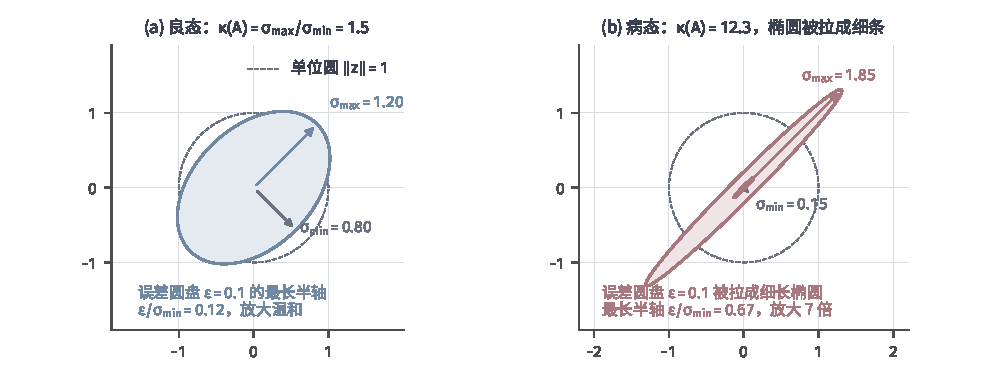
\includegraphics[width=169.0mm]{figures/00-shared/mathematical-preliminaries-upper/02-linear-spaces/matplotlib/ls-condition-number-amplification/ls-condition-number-amplification.pdf}
 \caption{条件数对误差圆盘的放大。灰虚线为单位圆$\lVert\bm z\rVert=1$；左为良态
 $\bm A_1=[[1,0.2],[0.2,1]]$，奇异值$1.20$与$0.80$，$\kappa_2=1.5$，像椭圆接近
 圆；右为病态$\bm A_2=[[1,0.85],[0.85,1]]$，奇异值$1.85$与$0.15$，$\kappa_2\approx12.3$，
 像被拉成细条。半径$\varepsilon=0.1$的误差圆盘（红）最长半轴为$\varepsilon/\sigma_{\min}$：
 良态为$0.125$，病态约$0.67$。}
 \label{fig:ls-condition-number-amplification}
\end{figure*}

把输入、输出都换成相对尺度，得到\term{相对条件数}（relative condition number）
\[
 \kappa_{\mathrm{rel}}(F;\bm z)
 =\lim_{\delta\to0}\ \sup_{0<\lVert\Delta\bm z\rVert\leq\delta}
 \frac{\lVert\Delta\bm y\rVert/\lVert F(\bm z)\rVert}
      {\lVert\Delta\bm z\rVert/\lVert\bm z\rVert}.
\]
对线性作用，$\kappa_{\mathrm{rel}}(\bm A;\bm x)=\lVert\bm A\rVert\lVert\bm x\rVert/\lVert\bm A\bm x\rVert$随$\bm x$变化：$\bm x$落在被压缩的方向上时，输出$\bm A\bm x$小，相对条件数大；落在主伸缩方向上时它小。对可逆方阵再对所有$\bm x$取最坏，令$\bm y=\bm A\bm x$，
\[
 \sup_{\bm x\neq\bm0}\frac{\lVert\bm A\rVert\lVert\bm x\rVert}{\lVert\bm A\bm x\rVert}
 =\lVert\bm A\rVert\sup_{\bm y\neq\bm0}\frac{\lVert\bm A^{-1}\bm y\rVert}{\lVert\bm y\rVert}
 =\lVert\bm A\rVert\,\lVert\bm A^{-1}\rVert ,
\]
这个只依赖矩阵的数就是矩阵的条件数。

\begin{definition}[可逆矩阵的条件数]
\label{def:matrix-analysis-condition-number}
对同一向量范数诱导的矩阵范数，可逆方阵$\bm A$的\term{条件数}（condition number）为
\begin{equation}
 \kappa(\bm A)=\lVert\bm A\rVert\,\lVert\bm A^{-1}\rVert .
 \label{eq:matrix-analysis-condition-number}
\end{equation}
\end{definition}
由第~\ref{sec:ls-svd}节，欧氏范数下$\lVert\bm A\rVert_2=\sigma_{\max}$、$\lVert\bm A^{-1}\rVert_2=1/\sigma_{\min}$，故
\begin{equation}
 \kappa_2(\bm A)=\frac{\sigma_{\max}(\bm A)}{\sigma_{\min}(\bm A)},
 \label{eq:matrix-analysis-spectral-condition-number}
\end{equation}
即最强放大与最弱放大之比。条件数总不小于$1$，因为$1=\lVert\bm I\rVert=\lVert\bm A\bm A^{-1}\rVert\leq\lVert\bm A\rVert\lVert\bm A^{-1}\rVert=\kappa(\bm A)$。正交矩阵的奇异值全为$1$，所以$\kappa_2=1$。矩阵接近奇异时$\sigma_{\min}\to0$，$\kappa_2$增大，与图~\ref{fig:ls-condition-number-amplification}右侧的细长椭圆一致。条件数接近$1$的问题称为良态，条件数很大的问题称为病态。

\begin{theorem}[条件数基本界]
\label{thm:matrix-analysis-condition-number-bound}
设$\kappa(F;\bm z)$为任务$F$在$\bm z$处的相对条件数，则足够小的输入扰动满足
\begin{equation}
 \frac{\lVert\Delta\bm y\rVert}{\lVert F(\bm z)\rVert}
 \lesssim\kappa(F;\bm z)\,\frac{\lVert\Delta\bm z\rVert}{\lVert\bm z\rVert}.
 \label{eq:matrix-analysis-condition-number-bound}
\end{equation}
特别地，可逆系统$\bm A\bm x=\bm b$的右端扰动$\Delta\bm b$引起的解扰动对任意大小的$\Delta\bm b$都满足$\lVert\Delta\bm x\rVert/\lVert\bm x\rVert\leq\kappa(\bm A)\lVert\Delta\bm b\rVert/\lVert\bm b\rVert$。
\end{theorem}
\begin{proof}
第一式是相对条件数定义的直接改写，$\lesssim$表示忽略比$\lVert\Delta\bm z\rVert$高阶的小量。对方程，$\bm A(\bm x+\Delta\bm x)=\bm b+\Delta\bm b$减去$\bm A\bm x=\bm b$，得$\Delta\bm x=\bm A^{-1}\Delta\bm b$，故$\lVert\Delta\bm x\rVert\leq\lVert\bm A^{-1}\rVert\lVert\Delta\bm b\rVert$；又$\lVert\bm b\rVert=\lVert\bm A\bm x\rVert\leq\lVert\bm A\rVert\lVert\bm x\rVert$，即$1/\lVert\bm x\rVert\leq\lVert\bm A\rVert/\lVert\bm b\rVert$。两式相乘即得。
\end{proof}

条件数是最坏方向上的上界，不是每个扰动都达到的倍数。一般任务的相对条件数只控制足够小的扰动；矩阵本身的扰动较大时，还要考虑扰动后是否仍然可逆，这在第~\ref{chap:linear-equations-and-optimization}章估计逆矩阵与方程解的敏感度时处理。

条件数也不回答反复作用的长期结果。下面的反例中，两个矩阵的条件数相同，幂的变化趋势却相反。
\begin{example}[反例：条件数相同而幂的趋势相反]
\label{ex:ls-condition-number-vs-powers}
给定同阶的$2\bm I$与$\tfrac12\bm I$。二者的奇异值分别全为$2$与全为$\tfrac12$，所以
\[
 \kappa_2(2\bm I)=\frac{2}{2}=1,\qquad
 \kappa_2\bigl(\tfrac12\bm I\bigr)=\frac{1/2}{1/2}=1 .
\]
但$(2\bm I)^k=2^k\bm I$逐次增长，$(\tfrac12\bm I)^k=2^{-k}\bm I$逐次衰减。结论：条件数相同的两个矩阵，反复作用的结果可以完全相反。
\end{example}
条件数衡量一次作用的相对放大，长期行为要由谱半径判断（第~\ref{sec:ls-matrix-power-behavior}节），二者不能互相代替。

\subsection{基本运算的敏感度}

同样的增量展开适用于第~\ref{chap:linear-operations}章的基本运算。先看加法。和的增量是$\Delta(\bm x+\bm y)=\Delta\bm x+\Delta\bm y$，由三角不等式，$\lVert\Delta(\bm x+\bm y)\rVert\leq\lVert\Delta\bm x\rVert+\lVert\Delta\bm y\rVert$，所以加法本身不放大绝对误差。但$\bm x\approx-\bm y$时理想输出很小，相对误差被小分母放大，下面的例子给出具体数值。
\begin{example}[加法中的抵消]
\label{ex:ls-cancellation-relative-error}
给定$x=1.0001$、$y=-1.0000$，二者各带至多$5\times10^{-5}$的绝对误差，相对误差约为$5\times10^{-5}$。理想和为$x+y=10^{-4}$，而和的绝对误差至多为$5\times10^{-5}+5\times10^{-5}=10^{-4}$，所以和的相对误差可达
\[
 \frac{10^{-4}}{10^{-4}}=1 .
\]
结论：输入的相对误差约为$5\times10^{-5}$，输出的相对误差却可达$1$，放大约$2\times10^4$倍。
\end{example}
这种抵消不是算法失误，而是问题本身在相对尺度下病态。

再看乘积。它满足
\[
 (\bm A+\bm E)(\bm B+\bm F)-\bm A\bm B=\bm A\bm F+\bm E\bm B+\bm E\bm F,
\]
前两项是一阶响应，各被另一个因子的范数放大，末项在小扰动下是二阶量。

最后看行列式，它在矩阵接近奇异时最敏感。
\begin{example}[接近奇异时的行列式]
\label{ex:ls-determinant-near-singular}
给定$\bm A=\operatorname{diag}(1,\varepsilon)$，$0<\varepsilon<1$，则$\det\bm A=\varepsilon$。把第二个对角元改为$\varepsilon+\delta$，矩阵的相对变化为$\lVert\Delta\bm A\rVert_2/\lVert\bm A\rVert_2=|\delta|$，行列式变为$\varepsilon+\delta$，相对变化为
\[
 \frac{|(\varepsilon+\delta)-\varepsilon|}{\varepsilon}=\frac{|\delta|}{\varepsilon}.
\]
结论：行列式的相对误差是矩阵相对误差的$1/\varepsilon$倍，矩阵越接近奇异，放大越强。
\end{example}

本节得到的结论是：条件数$\kappa(\bm A)=\lVert\bm A\rVert\lVert\bm A^{-1}\rVert$是一次作用下相对误差的最坏放大倍数，欧氏范数下等于$\sigma_{\max}/\sigma_{\min}$，在各方向伸缩悬殊、矩阵接近奇异时变大；加法在抵消时、行列式在矩阵接近奇异时，相对误差也会被小分母放大。这里矩阵始终是固定的，只有输入向量带误差。可是矩阵本身也常常来自数据，例如由有限样本估计的协方差矩阵。下一节把矩阵当作输入，研究它的特征值、奇异值与特征子空间对扰动的敏感度。

% 第6章第7节：谱的扰动（特征值与奇异值的移动、子空间之间的距离、特征子空间的转动）。

\section{谱的扰动}
\label{sec:ls-spectral-sensitivity}
\label{sec:linear-algebra-spectral-stability}
\label{sec:ch06-spectral-stability}

上一节让矩阵保持不变，只扰动输入向量。实际中矩阵本身也来自数据：协方差矩阵由有限样本估计，系数矩阵经过测量和舍入。这时谱分解的输入是矩阵，输出有两类：特征值（或奇异值）与特征子空间（或奇异子空间）。矩阵受到扰动$\bm E$后，它们分别移动多少？

本节先证明对称矩阵的特征值与任意矩阵的奇异值移动不超过$\lVert\bm E\rVert_2$，并说明非对称矩阵的特征值为何没有这样的保证；再建立一个与基的选取无关的子空间距离；最后证明特征子空间转过的角度由扰动与特征值间隔之比控制。

\subsection{特征值与奇异值的移动}
\label{sec:ls-spectral-value-sensitivity}

先看特征值。实对称矩阵的特征值全为实数，可以把扰动前后的特征值都按降序排列，记为$\lambda_1\geq\cdots\geq\lambda_d$与$\widetilde\lambda_1\geq\cdots\geq\widetilde\lambda_d$，再按同一次序逐个比较。对正定矩阵$\bm A$，椭圆$\{\bm x:\bm x^\top\bm A\bm x\leq1\}$的主轴沿特征方向，半轴长为$1/\sqrt\lambda$。图~\ref{fig:ls-perturbation-ellipse}画出$\bm A$换成$\bm A+\bm E$前后的两个椭圆：半轴长微变，主轴微转。

\begin{figure}[htbp]
 \centering
 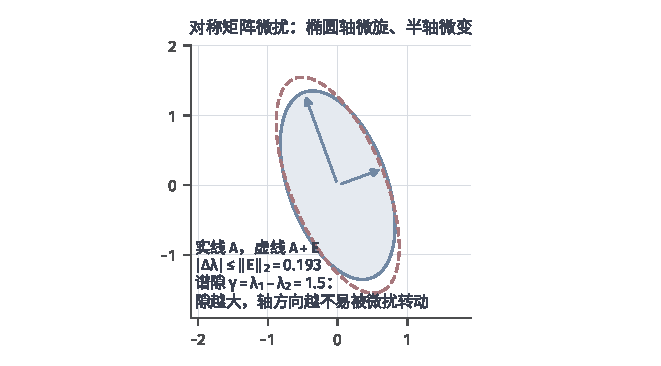
\includegraphics[width=112mm]{figures/00-shared/mathematical-preliminaries-upper/02-linear-spaces/matplotlib/ls-perturbation-ellipse/ls-perturbation-ellipse.pdf}
 \caption{对称矩阵微扰的谱与方向。实线椭圆为$\bm A$（特征值$2$与$0.5$，主轴
 方向$20^\circ$），虚线为$\bm A+\bm E$（$\lVert\bm E\rVert_2\approx0.193$）：轴
 微旋、半轴微变。新特征值约$2.18$与$0.37$，偏移$0.18$、$0.13$均小于
 $\lVert\bm E\rVert_2$，符合Weyl界；未扰动的谱隙$\delta=\lambda_1-\lambda_2=1.5$越大，
 特征方向越不易被微扰转动。}
 \label{fig:ls-perturbation-ellipse}
\end{figure}

Courant--Fischer定理把每个特征值写成Rayleigh商的最小最大值，而扰动$\bm E$对Rayleigh商的影响不超过$\lVert\bm E\rVert_2$，由此得到下面的界。
\begin{theorem}[Weyl特征值扰动界]
\label{thm:ls-weyl-eigenvalue}
对实对称$\bm A,\bm E\in\mathbb R^{d\times d}$，$\widetilde{\bm A}=\bm A+\bm E$与$\bm A$按降序配对的特征值满足
\begin{equation}
 |\widetilde\lambda_k-\lambda_k|
 \leq\lVert\bm E\rVert_2,
 \qquad k=1,\dots,d.
 \label{eq:matrix-analysis-weyl-eigenvalue-perturbation}
\end{equation}
\end{theorem}
\begin{proof}
$\bm E$对称，由Rayleigh--Ritz定理，它的Rayleigh商介于最小与最大特征值之间，而它们的绝对值不超过$\lVert\bm E\rVert_2$，所以$|\bm x^\top\bm E\bm x|\leq\lVert\bm E\rVert_2\lVert\bm x\rVert_2^2$。取$\mathcal V=\operatorname{span}\{\bm q_1,\ldots,\bm q_k\}$（$\bm A$的前$k$个特征向量），其中每个$\bm x$满足
\[
 \bm x^\top\widetilde{\bm A}\bm x=\bm x^\top\bm A\bm x+\bm x^\top\bm E\bm x\geq(\lambda_k-\lVert\bm E\rVert_2)\lVert\bm x\rVert_2^2 .
\]
由Courant--Fischer定理，$\widetilde\lambda_k$不小于$\widetilde{\bm A}$在任一$k$维子空间上Rayleigh商的最小值，故$\widetilde\lambda_k\geq\lambda_k-\lVert\bm E\rVert_2$。把$\widetilde{\bm A}$看作$\bm A$加扰动$-\bm E$，交换二者的角色得$\lambda_k\geq\widetilde\lambda_k-\lVert\bm E\rVert_2$。
\end{proof}

Weyl界不需要特征值彼此分开，单重与重复特征值都适用。

Weyl界也给出奇异值的稳定性。把$\bm A\in\mathbb R^{m\times d}$嵌入对称分块矩阵$\left[\begin{smallmatrix}\bm0&\bm A\\\bm A^\top&\bm0\end{smallmatrix}\right]$，由$\bm A\bm v_i=\sigma_i\bm u_i$、$\bm A^\top\bm u_i=\sigma_i\bm v_i$可直接验证向量$(\bm u_i,\pm\bm v_i)$是它的特征向量，特征值为$\pm\sigma_i$，其余特征值为零；而$\bm E$嵌入后谱范数不变。对嵌入矩阵应用Weyl界，得
\begin{equation}
 |\widetilde\sigma_i-\sigma_i|\leq\lVert\bm E\rVert_2 .
 \label{eq:matrix-analysis-singular-value-perturbation}
\end{equation}
截断SVD的误差$\sigma_{k+1}$（定理~\ref{thm:ls-best-low-rank}）因而也只移动不超过$\lVert\bm E\rVert_2$。

非对称矩阵的特征值没有这样的保证。设$\bm A=\bm V\bm\Lambda\bm V^{-1}$可对角化，$\mu$是$\bm A+\bm E$的特征值而不是$\bm A$的特征值，$\bm w$为对应的特征向量（必要时取复数）。由$(\bm A+\bm E)\bm w=\mu\bm w$，令$\bm y=\bm V^{-1}\bm w\neq\bm0$，得$(\bm\Lambda-\mu\bm I)\bm y=-\bm V^{-1}\bm E\bm V\bm y$。$\mu$不是$\bm A$的特征值，所以对角矩阵$\bm\Lambda-\mu\bm I$可逆，于是$\bm y=-(\bm\Lambda-\mu\bm I)^{-1}\bm V^{-1}\bm E\bm V\bm y$。两边取范数并除以$\lVert\bm y\rVert_2$，得$1\leq\lVert(\bm\Lambda-\mu\bm I)^{-1}\rVert_2\,\kappa_2(\bm V)\lVert\bm E\rVert_2$；而对角矩阵$(\bm\Lambda-\mu\bm I)^{-1}$的范数是$1/\min_k|\lambda_k-\mu|$，于是得到Bauer--Fike界
\[
 \min_k|\mu-\lambda_k|\leq\kappa_2(\bm V)\lVert\bm E\rVert_2 .
\]
特征向量越接近线性相关，$\kappa_2(\bm V)$越大，界越宽。对称情形$\bm V$可取正交矩阵，$\kappa_2(\bm V)=1$，界与Weyl界同量级。

不可对角化时情况更糟，特征值的移动可以远大于扰动本身。
\begin{example}[反例：特征值的移动远大于扰动]
\label{ex:ls-jordan-eigenvalue-sensitivity}
给定$\bm N=\left[\begin{smallmatrix}0&1\\0&0\end{smallmatrix}\right]$，它的特征值全为$0$。在左下角加入扰动$\varepsilon$，得
\[
 \bm N_\varepsilon=\begin{bmatrix}0&1\\\varepsilon&0\end{bmatrix},\qquad
 p_{\bm N_\varepsilon}(z)=z^2-\varepsilon ,
\]
扰动的大小为$\lVert\bm N_\varepsilon-\bm N\rVert_2=|\varepsilon|$。$\varepsilon>0$时特征值为$\pm\sqrt\varepsilon$，移动量为$\sqrt\varepsilon$；例如$\varepsilon=10^{-10}$时特征值移动$10^{-5}$，是扰动的$10^5$倍。$\varepsilon<0$时特征值为$\pm\mathrm i\sqrt{|\varepsilon|}$，实特征值消失。结论：特征值的移动量是$O(\sqrt{|\varepsilon|})$而非$O(|\varepsilon|)$，不能由扰动的范数乘一个常数控制。
\end{example}
可见对非对称矩阵，特征值的敏感程度取决于矩阵的结构：可对角化时，移动量至多是扰动的$\kappa_2(\bm V)$倍；不可对角化时，移动量甚至不与扰动成正比。

\subsection{子空间之间的距离}
\label{sec:ls-subspace-sensitivity}

比较特征向量时先要确定比较什么。同一子空间的基可以旋转、变号，单个基向量的变化不能当作子空间误差；特征值重复时，特征空间内部怎么换基都不改变子空间。所以比较对象必须是子空间本身，需要一个与基的选取无关的度量。图~\ref{fig:ls-principal-angles-subspaces}从两条过原点的直线看起：两直线的夹角与方向向量的选取无关；把一条直线的单位方向向量投影到另一条上，投影不掉的部分长度为$\sin\theta$。

\begin{figure}[htbp]
 \centering
 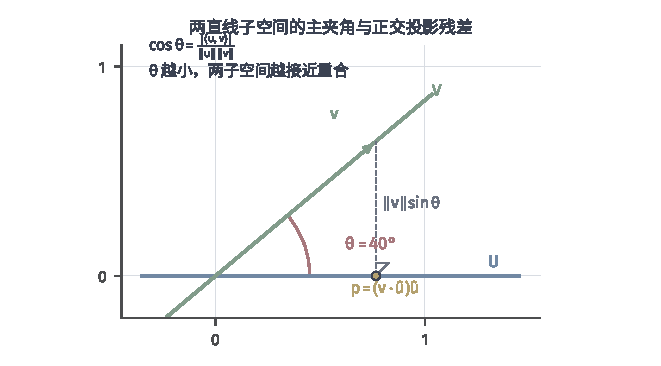
\includegraphics[width=112mm]{figures/00-shared/mathematical-preliminaries-upper/02-linear-spaces/matplotlib/ls-principal-angles-subspaces/ls-principal-angles-subspaces.pdf}
 \caption{两条直线子空间的主夹角。蓝线为$\bm U$、绿线为$\bm V$，红弧为主夹角
 $\theta=40^\circ$；黄点$\bm p$是$\bm v$在$\bm U$上的正交投影，灰虚线为投影
 垂线。$\cos40^\circ\approx0.766$、$\sin40^\circ\approx0.643$，残差长度
 $\lVert\bm v\rVert\sin\theta$即投影不掉的分量。}
 \label{fig:ls-principal-angles-subspaces}
\end{figure}

对一维子空间，若$\bm q,\widetilde{\bm q}$是单位方向向量，则$|\bm q^\top\widetilde{\bm q}|=\cos\theta$。高维子空间之间有多个夹角，由交叉内积矩阵的奇异值给出。
\begin{definition}[主夹角]
\label{def:matrix-analysis-principal-angles}
设$\bm Q,\widetilde{\bm Q}\in\mathbb R^{d\times r}$列标准正交，分别张成$r$维子空间。交叉矩阵$\bm Q^\top\widetilde{\bm Q}$的奇异值记为$\cos\theta_1\geq\dots\geq\cos\theta_r$，$0\leq\theta_1\leq\cdots\leq\theta_r\leq\pi/2$，这些$\theta_i$称为两个子空间的\term{主夹角}（principal angles）。
\end{definition}
这些奇异值都在$[0,1]$内，因为$\lVert\bm Q^\top\widetilde{\bm Q}\rVert_2\leq\lVert\bm Q\rVert_2\lVert\widetilde{\bm Q}\rVert_2=1$，所以$\theta_i$有定义。换基相当于把$\bm Q$、$\widetilde{\bm Q}$右乘正交矩阵，交叉矩阵的奇异值不变，所以主夹角只依赖子空间。

主夹角的正弦也可以直接读出。设$\widetilde{\bm Q}_\perp$的列是$\widetilde{\bm Q}$列空间正交补的标准正交基。对单位向量$\bm a$，把$\bm Q\bm a$分解到$\widetilde{\bm Q}$的列空间与其正交补，由勾股定理，
\[
 \lVert\widetilde{\bm Q}^\top\bm Q\bm a\rVert_2^2+\lVert\widetilde{\bm Q}_\perp^\top\bm Q\bm a\rVert_2^2=\lVert\bm Q\bm a\rVert_2^2=1 .
\]
记$\bm C=\widetilde{\bm Q}^\top\bm Q$、$\bm X=\widetilde{\bm Q}_\perp^\top\bm Q$。上式对所有单位向量$\bm a$成立，说明对称矩阵$\bm X^\top\bm X$与$\bm I-\bm C^\top\bm C$的二次型处处相等，所以$\bm X^\top\bm X=\bm I-\bm C^\top\bm C$。$\bm C$是交叉矩阵的转置，奇异值为$\cos\theta_i$，所以$\bm X^\top\bm X$的特征值是$1-\cos^2\theta_i=\sin^2\theta_i$，即$\bm X$的奇异值是$\sin\theta_i$。

子空间的误差还可以用正交投影$\bm P=\bm Q\bm Q^\top$、$\widetilde{\bm P}=\widetilde{\bm Q}\widetilde{\bm Q}^\top$之差表示，它与基的选取无关。可以证明
\[
 \lVert\bm P-\widetilde{\bm P}\rVert_2=\sin\theta_r,\qquad
 \tfrac12\lVert\bm P-\widetilde{\bm P}\rVert_{\mathrm F}^2=\sum_{i=1}^r\sin^2\theta_i .
\]
第二式可以直接验证：由$\operatorname{tr}\bm P=\operatorname{tr}\widetilde{\bm P}=r$与$\operatorname{tr}(\bm P\widetilde{\bm P})=\lVert\bm Q^\top\widetilde{\bm Q}\rVert_{\mathrm F}^2=\sum_i\cos^2\theta_i$，得$\lVert\bm P-\widetilde{\bm P}\rVert_{\mathrm F}^2=2r-2\sum_i\cos^2\theta_i=2\sum_i\sin^2\theta_i$。第一式说明投影矩阵之差的谱范数就是最大主夹角的正弦，它的证明较长，这里从略。

\subsection{特征子空间的转动}

有了主夹角，就可以估计扰动使特征子空间转过多大的角度。设$\bm A$、$\widetilde{\bm A}=\bm A+\bm E$实对称，$\bm Q$的列是$\bm A$的前$k$个单位特征向量，$\widetilde{\bm Q}$的列是$\widetilde{\bm A}$的前$k$个单位特征向量。要求目标特征值与扰动后其余特征值之间有间隔
\[
 \gamma=\lambda_k-\widetilde\lambda_{k+1}>0 .
\]
记$\widetilde{\bm Q}_\perp$为$\widetilde{\bm A}$其余特征向量组成的矩阵，$\widetilde{\bm\Lambda}_2$为对应的特征值对角矩阵，$\bm\Lambda_1=\operatorname{diag}(\lambda_1,\ldots,\lambda_k)$，并令$\bm X=\widetilde{\bm Q}_\perp^\top\bm Q$。由上一小节，它的奇异值就是两个子空间主夹角的正弦。

把$\widetilde{\bm Q}_\perp^\top\widetilde{\bm A}=\widetilde{\bm\Lambda}_2\widetilde{\bm Q}_\perp^\top$右乘$\bm Q$，把$\bm A\bm Q=\bm Q\bm\Lambda_1$左乘$\widetilde{\bm Q}_\perp^\top$，两式相减，由$\widetilde{\bm A}-\bm A=\bm E$得
\[
 \widetilde{\bm\Lambda}_2\bm X-\bm X\bm\Lambda_1=\widetilde{\bm Q}_\perp^\top\bm E\bm Q .
\]
这是关于$\bm X$的线性方程，两侧的系数矩阵都是对角的，因此可以逐元素求解（第~\ref{chap:linear-equations-and-optimization}章把形如$\bm A\bm X+\bm X\bm B=\bm C$的方程称为Sylvester方程）。逐元素写出为$(\widetilde\lambda_j-\lambda_i)X_{j,i}=(\widetilde{\bm Q}_\perp^\top\bm E\bm Q)_{j,i}$，其中$i\leq k<j$。由降序，$\lambda_i-\widetilde\lambda_j\geq\lambda_k-\widetilde\lambda_{k+1}=\gamma$，逐元素相除得
\[
 \lVert\bm X\rVert_{\mathrm F}\leq\frac{\lVert\widetilde{\bm Q}_\perp^\top\bm E\bm Q\rVert_{\mathrm F}}{\gamma}\leq\frac{\lVert\bm E\bm Q\rVert_{\mathrm F}}{\gamma}.
\]
左端的平方是主夹角正弦的平方和，所以这个平方和由扰动与谱隙之比控制。更细的论证给出谱范数下的同型结论，称为Davis--Kahan谱隙界\scite{math-golub2013matrix}：
\begin{equation}
 \lVert\widetilde{\bm P}-\bm P\rVert_2=\sin\theta_{k}
 \leq\frac{\lVert\bm E\rVert_2}{\gamma}.
 \label{eq:matrix-analysis-eigenvector-gap-bound}
\end{equation}
$\gamma$用到扰动后的特征值。若只知道未扰动的谱隙$\delta=\lambda_k-\lambda_{k+1}$，由Weyl界$\widetilde\lambda_{k+1}\leq\lambda_{k+1}+\lVert\bm E\rVert_2$，得$\gamma\geq\delta-\lVert\bm E\rVert_2$；当$\lVert\bm E\rVert_2\leq\delta/2$时，$\gamma\geq\delta/2$，右端不超过$2\lVert\bm E\rVert_2/\delta$。

谱隙在分母上：谱隙越小，子空间越容易被扰动转动。下面的二维例子可以精确算出转角。
\begin{example}[谱隙与特征方向的转角]
\label{ex:ls-gap-direction-rotation}
给定$\bm A_\alpha=\operatorname{diag}(\alpha,-\alpha)$（$\alpha>0$）与交叉扰动$\bm E=\varepsilon\left[\begin{smallmatrix}0&1\\1&0\end{smallmatrix}\right]$（$\varepsilon>0$）。$\bm A_\alpha$的两个特征值相距$2\alpha$，最大特征方向是$\bm e_1$。记$r=\sqrt{\alpha^2+\varepsilon^2}$，取$\theta\in(0,\pi/4)$满足$\cos2\theta=\alpha/r$、$\sin2\theta=\varepsilon/r$，即$\theta=\tfrac12\arctan(\varepsilon/\alpha)$。扰动后的矩阵可以写成
\[
 \bm A_\alpha+\bm E=\begin{bmatrix}\alpha&\varepsilon\\\varepsilon&-\alpha\end{bmatrix}
 =r\begin{bmatrix}\cos2\theta&\sin2\theta\\\sin2\theta&-\cos2\theta\end{bmatrix}.
\]
由两角差公式，
\[
 (\bm A_\alpha+\bm E)\begin{bmatrix}\cos\theta\\\sin\theta\end{bmatrix}
 =r\begin{bmatrix}\cos(2\theta-\theta)\\\sin(2\theta-\theta)\end{bmatrix}
 =r\begin{bmatrix}\cos\theta\\\sin\theta\end{bmatrix},
\]
而迹为零，另一个特征值是$-r$。所以最大特征方向从$\bm e_1$转到$(\cos\theta,\sin\theta)^\top$，转角为
\[
 \theta=\tfrac12\arctan\frac{\varepsilon}{\alpha}\approx\frac{\varepsilon}{2\alpha}\qquad(\varepsilon\ll\alpha).
\]
与界~\eqref{eq:matrix-analysis-eigenvector-gap-bound}比较：$\lVert\bm E\rVert_2=\varepsilon$，$\gamma=\lambda_1-\widetilde\lambda_2=\alpha+r\approx2\alpha$，界给出$\sin\theta\leq\varepsilon/\gamma\approx\varepsilon/(2\alpha)$，与实际转角同阶。结论：转角近似与谱隙$2\alpha$成反比，$\alpha$减半，转角加倍。
\end{example}
图~\ref{fig:matrix-analysis-gap-direction}画出这一关系。

谱隙只需存在于目标特征值组与组外之间，组内的特征值不必彼此分开。例如在$\operatorname{diag}(2,2,0)$中，特征值$2$对应的平面内每个单位向量都是特征方向，单独比较某个向量没有意义。但取$k=2$，未扰动的谱隙为$\delta=2-0=2$，由上面的推论，$\lVert\bm E\rVert_2\leq1$时整个二维特征子空间的最大主夹角满足$\sin\theta_2\leq2\lVert\bm E\rVert_2/\delta=\lVert\bm E\rVert_2$。

奇异子空间也有同样的结论。对第~\ref{sec:ls-spectral-value-sensitivity}节的对称嵌入矩阵$\left[\begin{smallmatrix}\bm0&\bm A\\\bm A^\top&\bm0\end{smallmatrix}\right]$作同样的谱隙论证，可知奇异子空间的稳定性由截断处的间隔$\sigma_k-\sigma_{k+1}$控制。所以截断SVD的误差$\sigma_{k+1}$总是稳定的，它所用的主方向却只在截断处有间隔时才稳定。

\begin{figure}
 \centering
 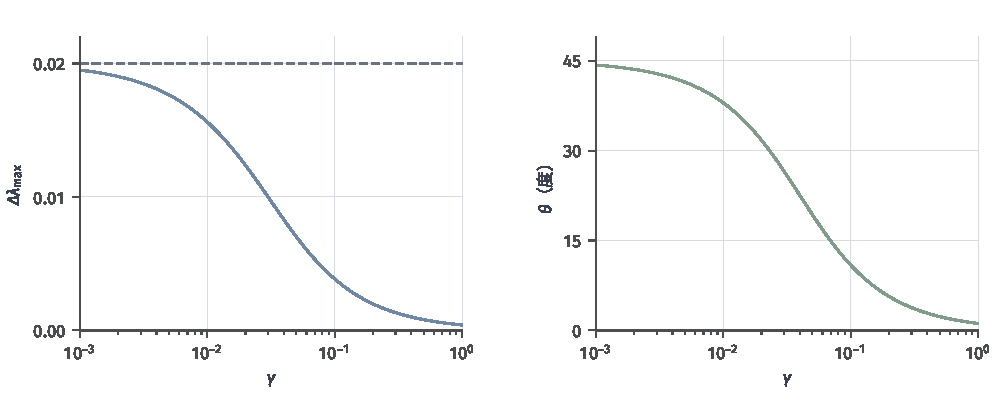
\includegraphics[width=0.92\linewidth]{figures/00-shared/mathematical-preliminaries-upper/02-linear-spaces/matplotlib/matrix-analysis-gap-direction/figure.pdf}
 \caption{谱隙方向示意：$\bm A_\alpha$的两个特征值相距$2\alpha$（谱隙），
 交叉扰动$\varepsilon$把最大特征方向转过约$\varepsilon/(2\alpha)$；
 谱隙越小，同样扰动转过的角度越大。}
 \label{fig:matrix-analysis-gap-direction}
\end{figure}

本节得到的结论是：把矩阵本身当作输入时，对称矩阵的特征值与任意矩阵的奇异值都是良态的，移动不超过$\lVert\bm E\rVert_2$，不要求特征值彼此分开；特征子空间要用与基无关的主夹角比较，它的转角由扰动与谱隙之比控制，谱隙越小越容易被转动；非对称矩阵的特征值可能对扰动非常敏感，敏感程度由特征向量矩阵的条件数或不可对角化的结构决定。条件数与谱的扰动讨论的都是一次作用或一次分解。下一节转向同一个矩阵的反复作用。

% 第6章第8节：矩阵的长期作用（谱半径判据、衰减速度与边界情形、瞬态放大、Neumann级数）。

\section{矩阵的长期作用}
\label{sec:ls-convergence}
\label{sec:linear-algebra-convergence-approximation}
\label{sec:ls-matrix-power-behavior}
\label{sec:linear-algebra-power-convergence}

条件数衡量的是一次作用的放大。迭代法、离散动态系统和许多学习算法却反复施加同一个线性作用，得到序列$\bm x^{(k)}=\bm A^k\bm x^{(0)}$；把这些作用累加起来，又得到矩阵级数。本节回答两个问题。第一，矩阵幂什么时候对所有初值都趋于零，趋近得多快，途中会不会先变大？第二，由矩阵幂组成的级数什么时候收敛，收敛到什么？

讨论收敛时不必担心范数的选择。第~\ref{sec:ls-finite-dimensional-sequences}节已经说明，有限维空间上的任意两个范数彼此等价（定理~\ref{thm:ls-norm-equivalence}），向量或矩阵序列是否收敛与所用范数无关，换范数只改变不等式中的常数。所以下面可以在任意方便的范数下论证，结论对所有范数成立。我们将看到，长期行为由谱半径决定，早期的放大则取决于矩阵是否正规。

\subsection{谱半径判据}

对固定方阵$\bm A$反复作用，初值$\bm x^{(0)}$在第$k$步变成$\bm x^{(k)}=\bm A^k\bm x^{(0)}$。只检查一个初值的轨迹不够：若初值恰好不含某个增长方向的分量，轨迹看起来收敛，换一个初值就发散。下面的反例说明这一点。
\begin{example}[反例：收敛与发散的轨迹]
\label{ex:ls-partial-convergence}
给定$\bm A=\operatorname{diag}(0.5,2)$，比较两个初值的轨迹：
\[
 \bm A^k\begin{bmatrix}1\\0\end{bmatrix}=\begin{bmatrix}0.5^k\\0\end{bmatrix}\to\bm0,\qquad
 \bm A^k\begin{bmatrix}0\\1\end{bmatrix}=\begin{bmatrix}0\\2^k\end{bmatrix},
\]
其中后一条轨迹的长度为$2^k\to\infty$。
结论：初值$(1,0)^\top$不含增长方向$\bm e_2$的分量，轨迹收敛；初值$(0,1)^\top$的轨迹发散。一个初值的轨迹收敛，不能说明矩阵幂趋于零。
\end{example}
所以要问的是：何时对全体初值都有$\bm A^k\bm x^{(0)}\to\bm0$？逐个取$\bm x^{(0)}=\bm e_j$可知，这等价于$\bm A^k$的每一列趋于零，即$\bm A^k\to\bm0$。

图~\ref{fig:ls-spectral-radius-convergence}显示了最简单的正规情形：误差每步乘以$\rho$，$\rho<1$时衰减，$\rho>1$时增长。

\begin{figure*}[htbp]
 \centering
 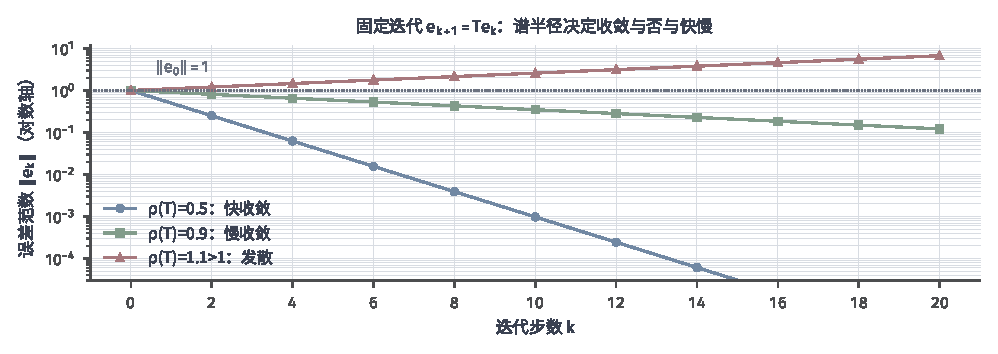
\includegraphics[width=169.0mm]{figures/00-shared/mathematical-preliminaries-upper/02-linear-spaces/matplotlib/ls-spectral-radius-convergence/ls-spectral-radius-convergence.pdf}
 \caption{谱半径决定迭代的长期方向。递推$\bm e^{(t+1)}=\bm A\bm e^{(t)}$、
 $\lVert\bm e^{(0)}\rVert=1$，取正规矩阵$\bm A=\rho\bm I$时$\lVert\bm e^{(t)}\rVert=\rho^t$：
 $\rho=0.5$（蓝）约十四步降到$10^{-4}$，$\rho=0.9$（绿）缓慢下降，
 $\rho=1.1$（红）指数上升。纵轴为半对数。}
 \label{fig:ls-spectral-radius-convergence}
\end{figure*}

最先想到的判据来自范数。由次乘性，$\lVert\bm A^k\rVert\leq\lVert\bm A\rVert^k$，所以只要在某个次乘性矩阵范数下$\lVert\bm A\rVert<1$，就有$\bm A^k\to\bm0$。但这只是充分条件：示例~\ref{ex:ls-nonnormal-norm-radius}的矩阵$\left[\begin{smallmatrix}0.8&4\\0&0.5\end{smallmatrix}\right]$二范数大于$4$，而示例~\ref{ex:ls-triangular-power}已经算出它的幂按$0.8^k$与$0.5^k$趋于零，它的谱半径也只有$0.8$。正规矩阵的范数等于谱半径；非正规矩阵的Schur形中，非对角块以及不呈模长乘旋转形式的$2\times2$对角块都会使范数大于谱半径。下面的引理先用相似变换把每个对角块化为模长乘旋转，再用一次坐标缩放把非对角块压小，从而把谱半径变成一个可用的几何上界。

\begin{lemma}[矩阵幂的几何上界]
\label{lem:ls-power-geometric-bound}
对任意$r>\rho(\bm A)$，存在常数$C_r$，使$\lVert\bm A^k\rVert_2\leq C_rr^k$对所有$k\geq0$成立；等价地，存在一个向量范数，使$\bm A$在它诱导的矩阵范数下不超过$r$。
\end{lemma}
\begin{proof}
取实Schur形$\bm A=\bm Q\bm T\bm Q^\top$，设$\bm T$有$s$个对角块，第$i$块的特征值模长为$|\lambda_i|$。

先处理对角块。每个$2\times2$对角块$\bm T_{i,i}$有一对共轭特征值，按第~\ref{sec:ls-general-square-spectrum}节的论证，在复特征向量的实部、虚部组成的基下，它化为模长乘旋转：$\bm T_{i,i}=\bm P_i(|\lambda_i|\bm R_i)\bm P_i^{-1}$，$\bm R_i$为旋转矩阵；$1\times1$块取$\bm P_i=1$、$\bm R_i=\pm1$。

再压小非对角块。对$0<\varepsilon\leq1$，令分块对角矩阵
\[
 \bm D_\varepsilon=\operatorname{diag}(\varepsilon^{0}\bm P_1,\varepsilon^{1}\bm P_2,\ldots,\varepsilon^{s-1}\bm P_s).
\]
直接相乘，$\bm D_\varepsilon^{-1}\bm T\bm D_\varepsilon$的第$(i,j)$块为$\varepsilon^{j-i}\bm P_i^{-1}\bm T_{i,j}\bm P_j$：对角块是$|\lambda_i|\bm R_i$，二范数不超过$\rho(\bm A)$；$j>i$的块带有因子$\varepsilon^{j-i}\leq\varepsilon$，所以全部非对角块的Frobenius范数不超过$\varepsilon c$，其中$c$与$\varepsilon$无关。把矩阵拆成分块对角部分与非对角部分，得
\[
 \lVert\bm D_\varepsilon^{-1}\bm T\bm D_\varepsilon\rVert_2\leq\rho(\bm A)+\varepsilon c .
\]
取$\varepsilon$足够小，使右端不超过$r$。

最后换回原坐标。令$\bm M=\bm Q\bm D_\varepsilon$，则$\bm A=\bm M(\bm D_\varepsilon^{-1}\bm T\bm D_\varepsilon)\bm M^{-1}$，中间各对$\bm M^{-1}\bm M$相消，$\bm A^k=\bm M(\bm D_\varepsilon^{-1}\bm T\bm D_\varepsilon)^k\bm M^{-1}$，故
\[
 \lVert\bm A^k\rVert_2\leq\lVert\bm M\rVert_2\lVert\bm M^{-1}\rVert_2\,r^k ,
\]
取$C_r=\lVert\bm M\rVert_2\lVert\bm M^{-1}\rVert_2$即可。所求的向量范数取$\bm x\mapsto\lVert\bm M^{-1}\bm x\rVert_2$，它诱导的$\bm A$的范数等于$\lVert\bm M^{-1}\bm A\bm M\rVert_2=\lVert\bm D_\varepsilon^{-1}\bm T\bm D_\varepsilon\rVert_2\leq r$。
\end{proof}

有了这个上界，就能给出矩阵幂衰减的充要条件。
\begin{theorem}[矩阵幂的衰减判据]
\label{thm:ls-power-decay}
对实方阵$\bm A$，$\bm A^k\to\bm0$当且仅当$\rho(\bm A)<1$。
\end{theorem}
\begin{proof}
充分性：取$r$满足$\rho(\bm A)<r<1$，由引理，$\lVert\bm A^k\rVert_2\leq C_rr^k\to0$。必要性：设有特征值$|\lambda|\geq1$。若$\lambda$为实数，其特征向量$\bm v$满足$\lVert\bm A^k\bm v\rVert=|\lambda|^k\lVert\bm v\rVert\not\to0$；若$\lambda$非实，在对应的二维不变子空间中，$\bm A^k$在基$(\bm u,\bm w)$下的矩阵是$|\lambda|^k$乘一个旋转，$\bm A^k\bm u$的坐标长度为$|\lambda|^k\geq1$，不趋于零。两种情形都有$\bm A^k\not\to\bm0$。
\end{proof}

\subsection{衰减速度与边界情形}

判据只回答矩阵幂是否趋于零，同一论证还给出衰减速度。上界$\lVert\bm A^k\rVert\leq C_rr^k$对任意$r>\rho(\bm A)$成立；必要性证明中的特征方向（或不变平面）给出下界$\lVert\bm A^k\rVert\geq c\,\rho(\bm A)^k$，$c>0$为常数。两边开$k$次方，$C_r^{1/k}$与$c^{1/k}$都趋于$1$，于是$\rho(\bm A)\leq\liminf_k\lVert\bm A^k\rVert^{1/k}\leq\limsup_k\lVert\bm A^k\rVert^{1/k}\leq r$。令$r$趋于$\rho(\bm A)$，得到Gelfand公式
\begin{equation}
 \rho(\bm A)=\lim_{k\to\infty}\lVert\bm A^k\rVert^{1/k}.
 \label{eq:ls-gelfand-formula}
\end{equation}
由范数等价（定理~\ref{thm:ls-norm-equivalence}），换成任意矩阵范数只改变常数，开$k$次方后常数的影响消失，所以公式对任意矩阵范数成立。由$\lVert\bm A^k\rVert\leq\lVert\bm A\rVert^k$还得$\rho(\bm A)\leq\lVert\bm A\rVert$对任意次乘性范数成立。

Gelfand公式说明，谱半径是每步放大倍数的长期几何平均：长期看，误差每步大约乘以$\rho(\bm A)$。由$\rho^m=1/10$解出，把误差缩小$10$倍约需$m=1/\log_{10}(1/\rho)$步，$\rho=0.5$时约$3.3$步，$\rho=0.99$时约$229$步；$\rho$越接近$1$，收敛越慢。

$\rho(\bm A)=1$是边界情形，结果取决于模为$1$的特征值。特征值$1$的特征方向保持不动，$-1$的特征方向来回翻转，模为$1$的非实特征值对应纯旋转；在这些方向上$\bm A^k$不趋于零，但保持有界。若模为$1$的特征值缺少足够的特征向量，还会出现增长。
\begin{example}[反例：谱半径为$1$而矩阵幂无界]
\label{ex:ls-unit-spectral-radius-growth}
给定$\bm J_1=\left[\begin{smallmatrix}1&1\\0&1\end{smallmatrix}\right]$，它只有特征值$1$，$\rho(\bm J_1)=1$，特征向量只有$(1,0)^\top$的倍数。按示例~\ref{ex:ls-jordan-block-power}的二项式展开，把$0.8$换成$1$，得
\[
 \bm J_1^k=(\bm I+\bm N)^k=\bm I+k\bm N=\begin{bmatrix}1&k\\0&1\end{bmatrix}.
\]
结论：右上角随$k$线性增长，$\lVert\bm J_1^k\rVert_2\geq k\to\infty$；谱半径等于$1$不能保证矩阵幂有界。
\end{example}
$\rho(\bm A)>1$时，由定理~\ref{thm:ls-power-decay}必要性的证明，从模大于$1$的特征值的特征方向（或不变平面）出发的轨迹不趋于零；但如示例~\ref{ex:ls-partial-convergence}所示，不必每个初值都发散。

\subsection{非正规矩阵的瞬态放大}

$\rho(\bm A)<1$保证最终衰减，但不说明途中的情况。下面的例子中，轨迹先变长、后衰减。
\begin{example}[非正规矩阵的瞬态放大]
\label{ex:ls-transient-growth}
给定迭代
\begin{equation}
 \bm A=\begin{bmatrix}0.8&4\\0&0.5\end{bmatrix},\qquad
 \bm x^{(k+1)}=\bm A\bm x^{(k)},\qquad \bm x^{(0)}=(0,1)^{\top}.
 \label{eq:ch06-fixed-iteration-example}
\end{equation}
示例~\ref{ex:ls-triangular-power}已把初值沿特征向量$\bm v_1=(1,0)^{\top}$、$\bm v_2=(-40/3,1)^{\top}$分解为$\bm x^{(0)}=\tfrac{40}{3}\bm v_1+\bm v_2$，并写出了矩阵幂与轨迹：
\begin{equation}
 \bm A^k=
 \begin{bmatrix}
  0.8^k&\frac{40}{3}(0.8^k-0.5^k)\\
  0&0.5^k
 \end{bmatrix},\qquad
 \bm x^{(k)}=
 \begin{bmatrix}\frac{40}{3}(0.8^k-0.5^k)\\0.5^k\end{bmatrix}.
 \label{eq:ch06-diagonalizable-finite-trajectory}
\end{equation}
代入$k=1,2,3$得
\[
 \bm x^{(1)}=\begin{bmatrix}4\\0.5\end{bmatrix},\qquad
 \bm x^{(2)}=\begin{bmatrix}5.2\\0.25\end{bmatrix},\qquad
 \bm x^{(3)}=\begin{bmatrix}5.16\\0.125\end{bmatrix},
\]
长度分别约为$4.03$、$5.21$、$5.16$，都远大于初值的长度$1$。另一方面$\rho(\bm A)=0.8<1$，由定理~\ref{thm:ls-power-decay}，轨迹最终趋于零。结论：谱半径小于$1$时，轨迹仍可以先放大数倍、再衰减。
\end{example}
放大的原因在于初值的分解。$\tfrac{40}{3}\bm v_1=(40/3,0)^\top$与$\bm v_2=(-40/3,1)^\top$都很长、方向几乎相反，初值$(0,1)^\top$由二者相消而成。两个分量衰减速度不同，相消很快被打破，所以长度先增后降（图~\ref{fig:ch06-transient-growth}）。

\begin{figure*}[htbp]
  \centering
  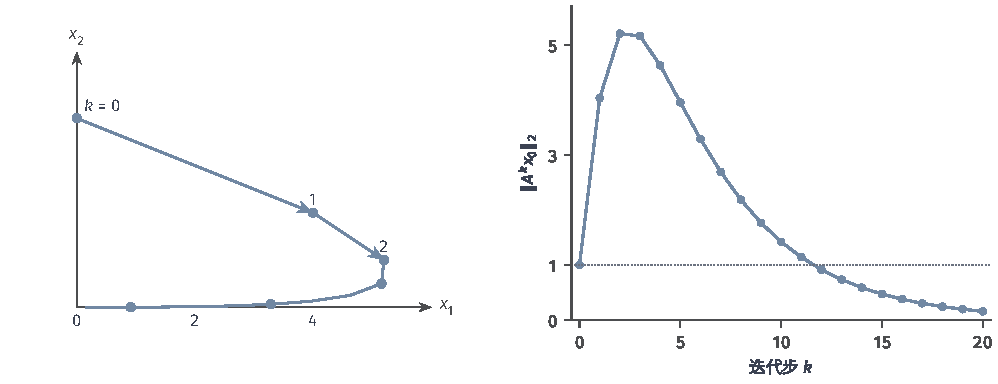
\includegraphics[width=169.0mm]{figures/00-shared/mathematical-preliminaries-upper/02-linear-spaces/matplotlib/ch06-transient-growth/figure.pdf}
  \caption{固定二维矩阵的反复作用。初值为$(0,1)^{\top}$，前两步的长度增加，
  此后回到原点；右图将长度与初始长度$1$比较。特征值$0.8$和$0.5$决定长期衰减，
  非正交特征方向间的相消则决定早期放大。两图使用同一个矩阵和同一组迭代点。}
  \label{fig:ch06-transient-growth}
\end{figure*}

一般地，可对角化矩阵$\bm A=\bm V\bm\Lambda\bm V^{-1}$满足$\bm A^k=\bm V\bm\Lambda^k\bm V^{-1}$，所以
\[
 \lVert\bm A^k\rVert_2\leq\lVert\bm V\rVert_2\lVert\bm V^{-1}\rVert_2\,\rho(\bm A)^k .
\]
特征向量越接近线性相关，$\lVert\bm V\rVert_2\lVert\bm V^{-1}\rVert_2$越大，早期可能的放大越强。正规矩阵则满足$\lVert\bm A^k\rVert_2=\rho(\bm A)^k$（第~\ref{sec:ls-general-square-spectrum}节），不会出现瞬态放大。

不可对角化时，特征向量本身就不够，矩阵幂中还会出现多项式因子。考虑$s$阶矩阵$\bm J=\lambda\bm I+\bm N$，其中$\bm N$是超对角元为$1$、其余元素为零的矩阵，满足$\bm N^s=\bm0$；这样的矩阵称为Jordan块，示例~\ref{ex:ls-jordan-block-power}的$\bm J$是$s=2$的情形。$\lambda\bm I$与$\bm N$可交换，二项式展开成立，且$j\geq s$的项为零：
\begin{equation}
 \bm J^k=\sum_{j=0}^{\min(k,s-1)}\binom{k}{j}\lambda^{k-j}\bm N^j .
 \label{eq:ch06-jordan-power}
\end{equation}
$\binom kj$是$k$的至多$s-1$次多项式，而多项式增长慢于几何衰减，$k^{s-1}|\lambda|^k\to0$（$|\lambda|<1$）。所以$|\lambda|<1$时块幂仍趋于零，只是起初可能上升。下面用二阶块看这种先升后降。
\begin{example}[Jordan块幂的先升后降]
\label{ex:ls-jordan-transient}
给定$\bm J=\left[\begin{smallmatrix}0.8&1\\0&0.8\end{smallmatrix}\right]$与初值$(0,1)^{\top}$。由示例~\ref{ex:ls-jordan-block-power}，
\[
 \bm J^k\begin{bmatrix}0\\1\end{bmatrix}=\begin{bmatrix}k\,0.8^{k-1}\\0.8^k\end{bmatrix}.
\]
第一坐标在$k=1,2,\ldots,6$时依次为$1$、$1.6$、$1.92$、$2.048$、$2.048$、$1.966$（末项保留三位小数），在$k=4,5$时达到最大值约$2.05$，此后才衰减。结论：特征值$0.8<1$保证最终衰减，但多项式因子$k$使第一坐标先上升到初值长度的两倍以上。
\end{example}
图~\ref{fig:vol1-add-linear-jordan-accumulation}画出这条轨迹的两个坐标。多项式因子也是引理~\ref{lem:ls-power-geometric-bound}中常数$C_r$的来源：$r$越接近$\rho(\bm A)$，需要的$\varepsilon$越小，$C_r$可能越大。

\begin{figure}[!htb]
  \centering
  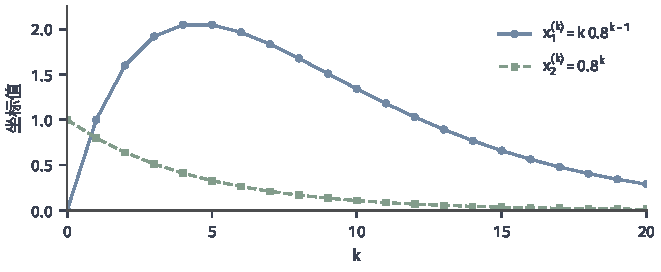
\includegraphics[width=112mm]{figures/00-shared/mathematical-preliminaries-upper/02-linear-spaces/matplotlib/comprehension-additions/linear-jordan-accumulation.pdf}
  \caption{Jordan块的累积项。取正文$\bm J=\left[\begin{smallmatrix}0.8&1\\0&0.8\end{smallmatrix}\right]$与初值$(0,1)^{\top}$。绿线为$0.8^k$，蓝线在$k\geq1$时为$k0.8^{k-1}$，在$k=0$时为$0$。点表示整数步，连线仅引导读图；两坐标最终都趋零。}
  \label{fig:vol1-add-linear-jordan-accumulation}
\end{figure}

所以报告迭代的收敛性时，要分开两件事：谱半径给出长期速度，特征向量的病态程度或Jordan块决定早期可能的放大。

\subsection{Neumann级数}
\label{sec:ls-matrix-series-exponential}

把矩阵幂累加起来会得到什么？最常用的是$\sum_k\bm A^k$，它把求逆$(\bm I-\bm A)^{-1}$写成反复作用之和，也描述每步注入的误差怎样累积。这里说矩阵级数$\sum_{k=0}^{\infty}\bm A^k$收敛，指部分和$\bm S_N=\sum_{k=0}^N\bm A^k$作为矩阵序列收敛。对标量$a$，$|a|<1$时几何级数$\sum_ka^k=1/(1-a)$；矩阵情形有同样的结论。

\begin{theorem}[Neumann级数与逆]
\label{thm:ls-neumann}
若在某个次乘性矩阵范数下$\lVert\bm A\rVert<1$，则级数$\sum_{k=0}^{\infty}\bm A^k$收敛，$\bm I-\bm A$可逆，且
\begin{equation}
 (\bm I-\bm A)^{-1}=\sum_{k=0}^{\infty}\bm A^k,
 \label{eq:ls-neumann-series}
\end{equation}
截断尾项满足$\lVert\sum_{k>N}\bm A^k\rVert\leq\lVert\bm A\rVert^{N+1}/(1-\lVert\bm A\rVert)$。
\end{theorem}
\begin{proof}
由次乘性，$\sum_k\lVert\bm A^k\rVert\leq\sum_k\lVert\bm A\rVert^k<\infty$。由范数等价（定理~\ref{thm:ls-norm-equivalence}），每个元素的绝对值不超过常数乘$\lVert\bm A^k\rVert$，所以每个元素的级数绝对收敛，矩阵级数收敛到某个$\bm S$；尾界由几何级数求和得到。逐项相消，$(\bm I-\bm A)\bm S_N=\bm S_N(\bm I-\bm A)=\bm I-\bm A^{N+1}$，令$N\to\infty$，$\bm A^{N+1}\to\bm0$，得$(\bm I-\bm A)\bm S=\bm S(\bm I-\bm A)=\bm I$。
\end{proof}
条件$\lVert\bm A\rVert<1$可以放宽到谱半径。由引理~\ref{lem:ls-power-geometric-bound}，只要$\rho(\bm A)<1$，就存在使$\lVert\bm A\rVert<1$的诱导范数，所以级数在$\rho(\bm A)<1$时收敛，只是尾界要在那个范数中读取；反之$\rho(\bm A)\geq1$时，由定理~\ref{thm:ls-power-decay}，通项$\bm A^k$不趋于零，级数发散。图~\ref{fig:ls-neumann-series-tail}用一个$2\times2$例子核对尾界。

\begin{figure}[htbp]
 \centering
 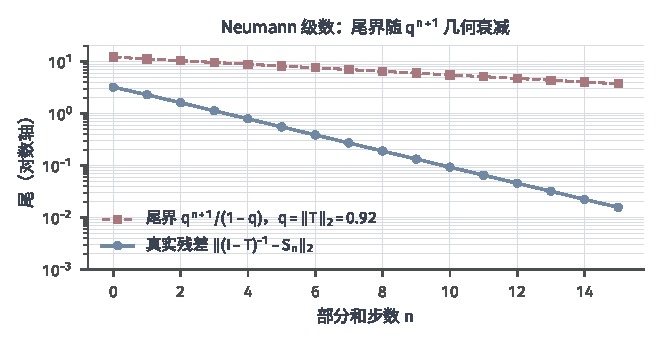
\includegraphics[width=112mm]{figures/00-shared/mathematical-preliminaries-upper/02-linear-spaces/matplotlib/ls-neumann-series-tail/ls-neumann-series-tail.pdf}
 \caption{Neumann级数尾界。$\bm T=[[0.7,0.6],[0,0.1]]$，$q=\lVert\bm T\rVert_2
 \approx0.924<1$，$(\bm I-\bm T)^{-1}=\sum\bm T^k$。蓝线为真实残差
 $\lVert\bm R_n\rVert=\lVert\bm T^{n+1}(\bm I-\bm T)^{-1}\rVert$，红虚线为尾界
 $q^{n+1}/(1-q)$，纵轴半对数（$n=0,\dots,15$）。}
 \label{fig:ls-neumann-series-tail}
\end{figure}

\paragraph{持续扰动的累积}

同样的级数描述持续扰动的累积。迭代的每一步都可能引入新误差（例如舍入），递推成为$\bm e^{(t+1)}=\bm T\bm e^{(t)}+\bm\delta^{(t)}$，$\bm\delta^{(t)}$是第$t$步注入的误差。逐步展开，
\[
 \bm e^{(t)}=\bm T^t\bm e^{(0)}+\sum_{j=0}^{t-1}\bm T^{t-1-j}\bm\delta^{(j)} .
\]
若在某个范数下$\lVert\bm T\rVert\leq q<1$且$\lVert\bm\delta^{(j)}\rVert\leq\delta$，第二项不超过$\delta\sum_{i\geq0}q^i$，于是
\begin{equation}
 \lVert\bm e^{(t)}\rVert\leq q^t\lVert\bm e^{(0)}\rVert+\frac{\delta}{1-q}.
 \label{eq:ls-noise-floor}
\end{equation}
初始误差几何衰减，持续扰动却留下不随$t$下降的误差下限$\delta/(1-q)$；$q$越接近$1$，下限越高。

本节的两个问题至此都有了回答。矩阵幂对全体初值衰减，当且仅当谱半径小于$1$；谱半径还是每步放大倍数的长期几何平均，决定收敛快慢。非正规矩阵在衰减之前可能先放大，放大程度由特征向量的病态程度或不可对角化的结构决定。Neumann级数在谱半径小于$1$时收敛到$(\bm I-\bm A)^{-1}$，持续注入的扰动则留下不随步数下降的误差下限。

% 第6章第9节：本章小结。

\section{本章小结}
\label{sec:ls-analysis-summary}
\label{sec:linear-algebra-summary}
\label{sec:matrix-analysis-summary}

本章围绕一个问题展开：同一个线性作用在什么样的基下最简单，从这个最简形式又能读出它的哪些性质？

前五节逐步调整对基的要求，回答前一半。由特征向量组成的基使矩阵成为对角形；特征值是特征多项式$p_{\bm A}(z)=\det(z\bm I-\bm A)$的根，不随基改变，Cayley--Hamilton定理说明$p_{\bm A}(\bm A)=\bm0$。$n$阶矩阵可对角化，当且仅当它有$n$个线性无关的实特征向量，这时$\bm A^k=\bm V\bm\Lambda^k\bm V^{-1}$。要求基标准正交时，能对角化的恰好是对称矩阵，特征值因而是Rayleigh商的极值；一般方阵只能化为实Schur形，正规矩阵化为分块对角形。输入、输出各取一组标准正交基时，任何矩阵都有奇异值分解，它给出谱范数、Frobenius范数和最佳低秩逼近。

后三节用这些最简形式读出三类性质，它们相互关联而不能互相代替。一次作用的误差放大由条件数$\kappa_2=\sigma_{\max}/\sigma_{\min}$衡量；把矩阵本身当作输入时，对称矩阵的特征值与任意矩阵的奇异值移动不超过$\lVert\bm E\rVert_2$，特征子空间的转角由扰动与谱隙之比控制，非正规矩阵的特征值则可能很敏感；反复作用的长期速度由谱半径决定，$\bm A^k\to\bm0$当且仅当$\rho(\bm A)<1$，但非正规矩阵会先放大再衰减。第~\ref{chap:linear-equations-and-optimization}章求解线性方程、最小二乘与矩阵方程时，将用到奇异值分解、条件数、谱、Cayley--Hamilton定理与实Schur形。

